\documentclass{beamer}
\usepackage{amsfonts,amsmath,oldgerm}
\usetheme{_statale}
\usefonttheme[onlymath]{serif}

\usepackage{enumitem}
\usepackage[italian]{babel}
\usepackage{xcolor}
\usepackage{graphicx}

\usepackage{hyperref}
\newcommand{\hypercite}[2]{\href{#1}{\cite{#2}}}

\usepackage[backend=biber, style=authoryear]{biblatex}
\addbibresource{bibliografia.bib}

%\newcommand{\testcolor}[1]{\colorbox{#1}{\textcolor{#1}{test}}~\texttt{#1}}
%\newcommand{\hrefcol}[2]{\textcolor{cyan}{\href{#1}{#2}}}
\titlebackground*{assets/background}

\renewcommand{\figurename}{Figura}


\title{Il modello di Ising}
\course{Simulazione di Materia Condensata e Biosistemi}
\author{Filippo Negrini}
\IDnumber{Matricola: 47127A}
\date{}


\begin{document}
\maketitle

Il modello di Ising consiste in un reticolo che presenta un momento magnetico (o spin) in ogni sito. Nel 
modello questi spin assumono la forma più semplice possibile, non particolarmente realistica, di variabili 
scalari $\sigma_i$ di valori $\pm 1$, rappresentanti rispettivamente dipoli unitari rivolti verso l'alto oppure 
verso il basso. Tali spin interagiscono fra loro e possono accoppiarsi ad un campo magnetico esterno e 
per tale motivo l'Hamiltoniana del sistema assume la forma 

\begin{equation}
    H\,=\,-J\sum_{\left<ij\right>} \sigma_i \sigma_j\,-\,h\sum_{i} \sigma_i,
    \label{eq: ising_ham}
\end{equation}

dove la notazione $\left<ij\right>$ denota una somma su primi vicini. Se il parametro $J$ è positivo i dipoli vicini 
tendono ad allinearsi e quindi il modello è di tipo ferromagnetico, altrimenti quando $J\,<\,0$ si ha anti-allineamento 
e fenomenologia anti-ferromagnetica.
\section{Metodi numerici}

%-----------------------------------------%
%				Prima slide				  %
%	        Metropolis vs Wolff     	  %
%-----------------------------------------%
\begin{frame}
    \frametitle{Metropolis vs Wolff}
    \framesubtitle{}

    \begin{columns}

        \begin{column}{0.5\textwidth}
            \begin{block}{Metropolis}

                \begin{itemize}[itemsep=0.5em, label=$\diamond$]
                    \item Tentata inversione di un singolo spin
                    \item $A\left(\nu\,|\,\mu\right)\,=\,\text{min}\left[1,\,e^{-\beta\left(E_{\nu}\,-\,E_{\mu}\right)}\right]$
                    \item Ottimo per $T \ll T_c$ oppure $T \gg T_c$
                \end{itemize}

                \centering
                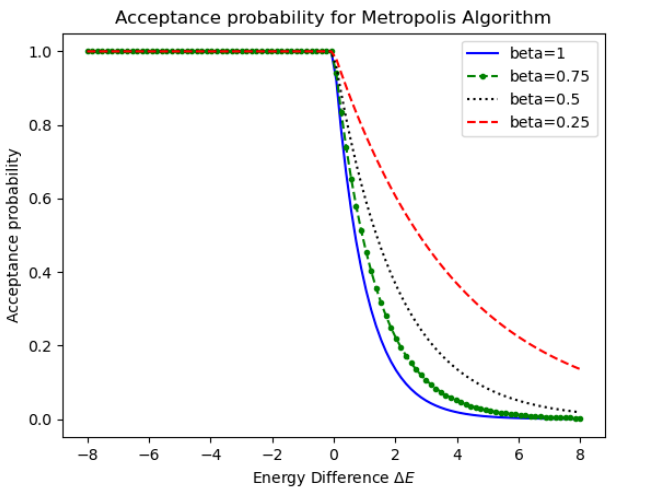
\includegraphics[width=0.9\textwidth]{Immagini/metodiNumerici/accRate_metro.png}	
                
            \end{block}
        \end{column}


        \begin{column}{0.5\textwidth}
            \begin{block}{Wolff}

                \begin{itemize}[itemsep=0.5em, label=$\diamond$]
                    \item Algoritmo di clustering
                    \item $P_{add}\,=\,1\,-\,\exp{\left(-2\beta J\right)}$
                    \item Ottimo per $T \simeq T_c$
                \end{itemize}

                \centering
                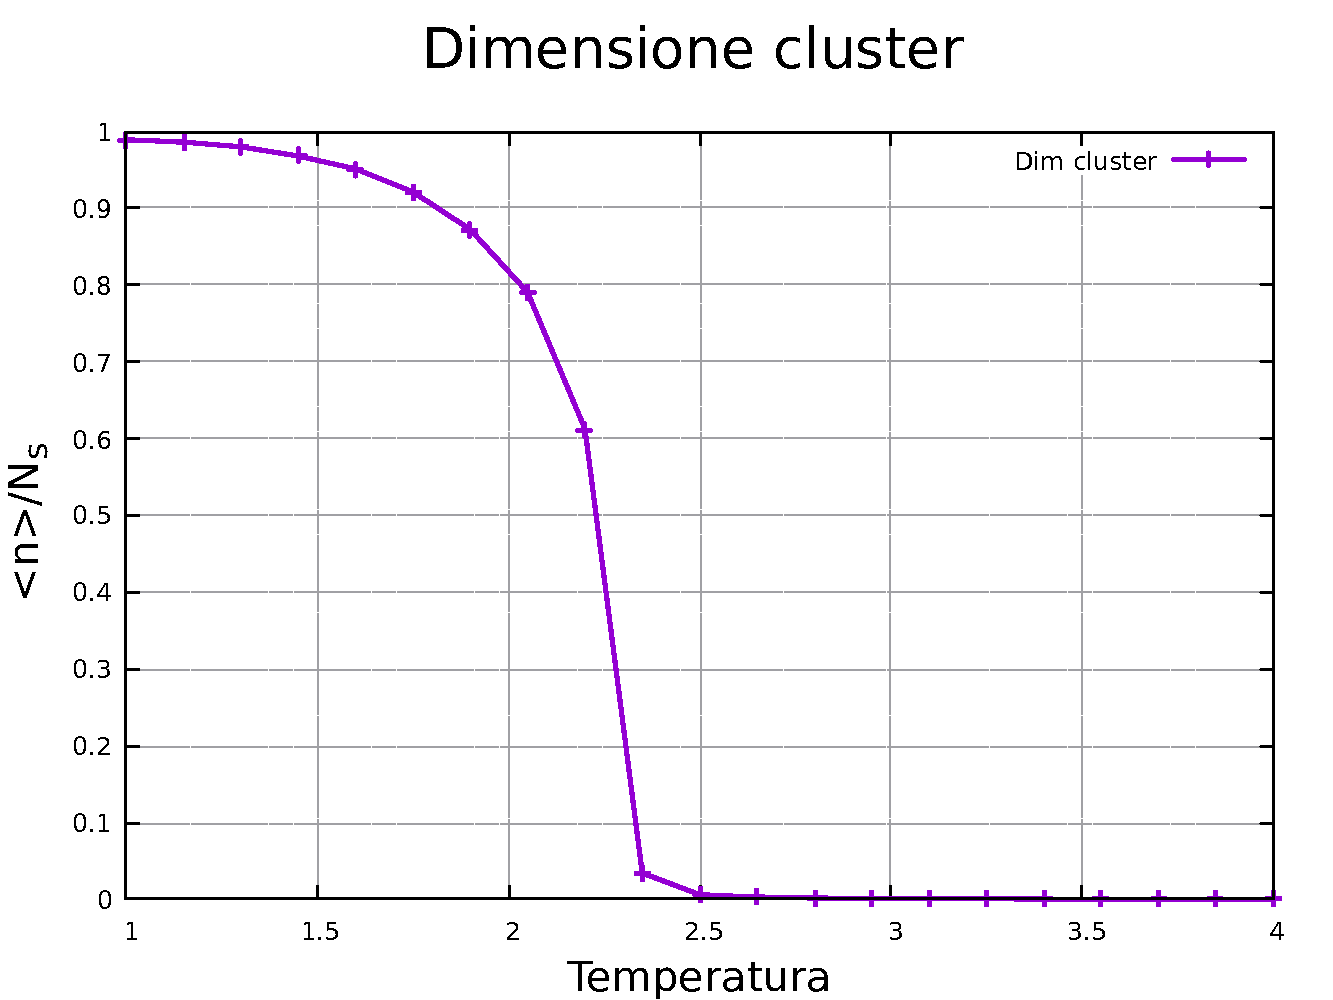
\includegraphics[width=0.7\textwidth]{Immagini/metodiNumerici/dimClFlip.pdf}			
            
            \end{block}
        \end{column}
      \end{columns}
  
\end{frame}



%-----------------------------------------%
%		       Seconda slide		      %
%       Termalizzazione del modello       %
%-----------------------------------------%
\begin{frame}
    \frametitle{Termalizzazione}
    \framesubtitle{}

    \begin{columns}

        \begin{column}{0.6\textwidth}

            \centering
            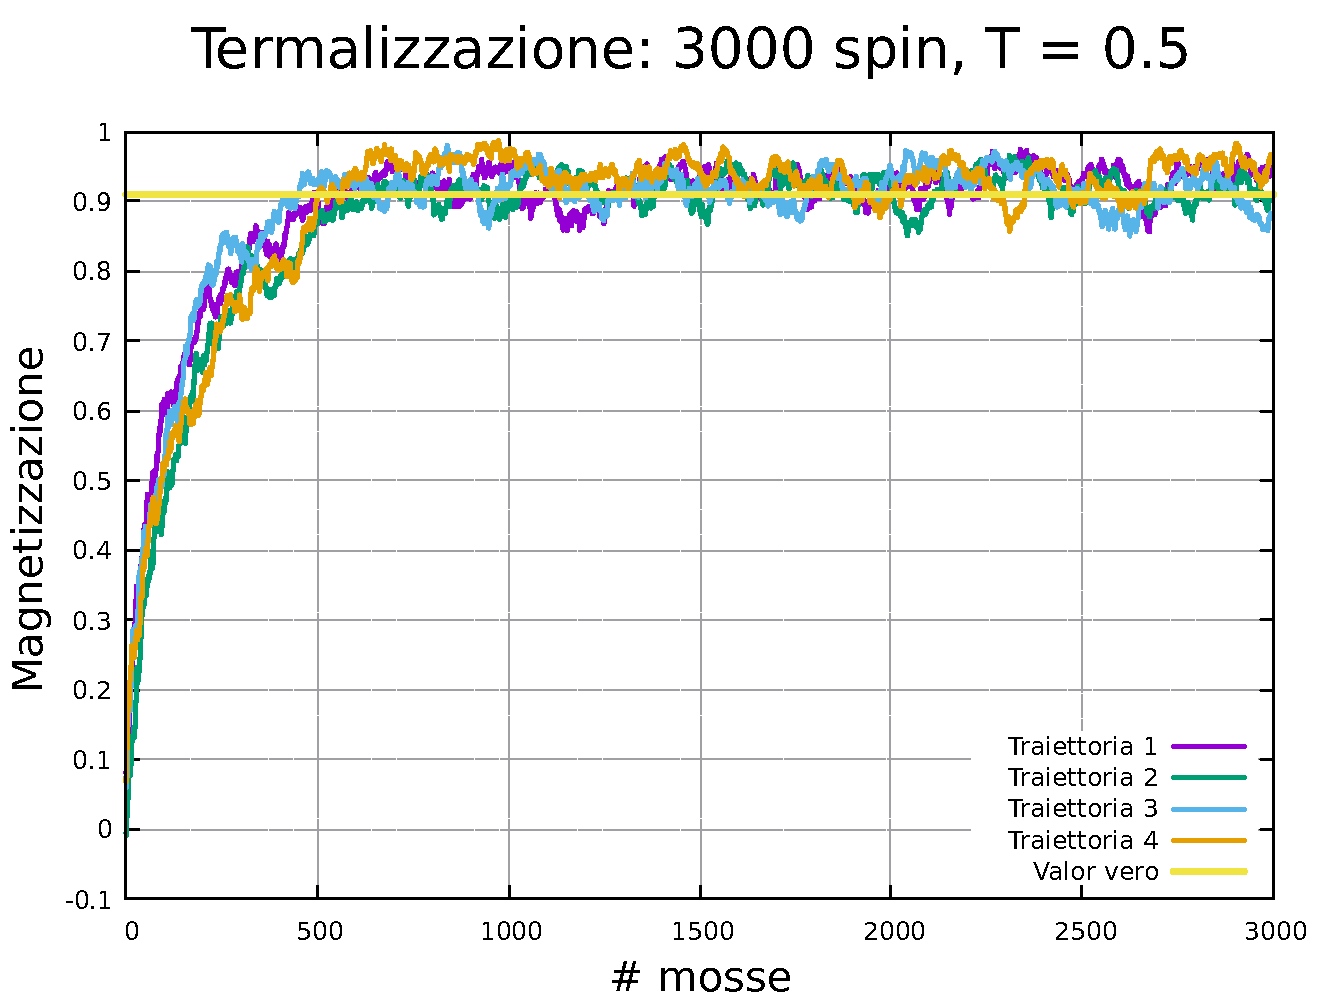
\includegraphics[width=\textwidth]{Immagini/metodiNumerici/term_3000_0.5.pdf}
            \newline
            {\scriptsize Termalizzazione per modello di Ising 1D.}

        \end{column}


        \begin{column}{0.4\textwidth}
            
            \begin{itemize}[itemsep=0.5em, label=$\diamond$]
                \item Giungere all'equilibrio termodinamico
                \item Attenzione a stati metastabili
                \item Dipendenza dalla condizione iniziale
            \end{itemize}
            
        \end{column}
      \end{columns}
  
\end{frame}



%-------------------------------------------%
%		        Terza slide	        	    %
%  Autocorrelazione e tempi caratteristici  %
%-------------------------------------------%
\begin{frame}
    \frametitle{Auto-correlazione}
    \framesubtitle{}

    \begin{columns}

        \begin{column}{0.55\textwidth}

            \centering
            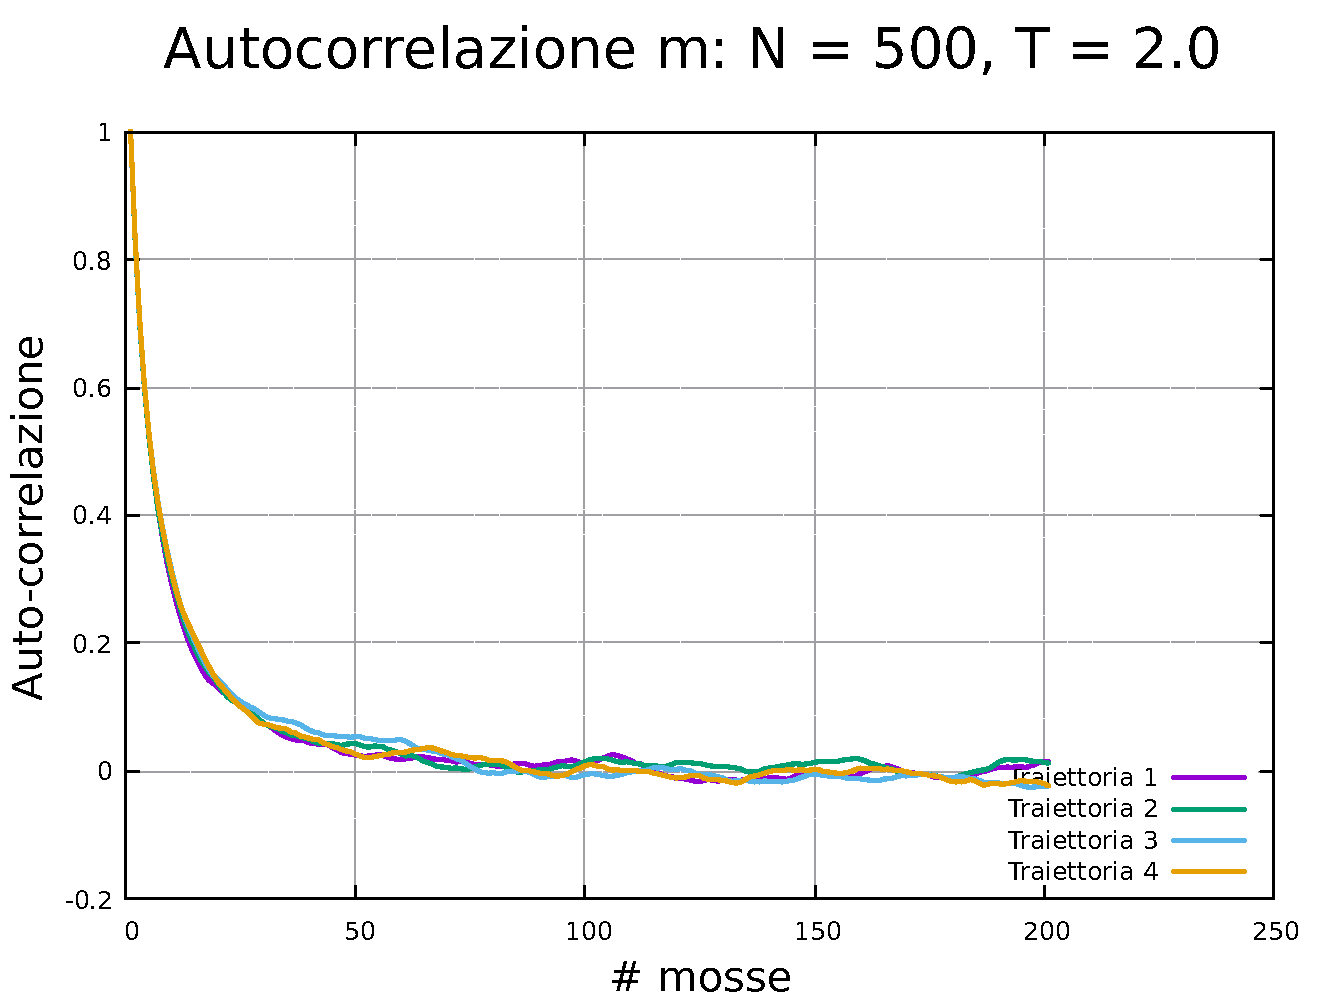
\includegraphics[width=\textwidth]{Immagini/metodiNumerici/auto_500_2.0.pdf}
            \newline
            {\scriptsize Autocorrelazione per modello di Ising 2D.}

        \end{column}


        \begin{column}{0.45\textwidth}

            \begin{block}{Definizione}
                \centering
                $\chi\left(t\right)\,=\,\frac{\left<m\left(t'\right)m\left(t'\,+\,t\right)\right>_{t'}\,-\,\left<m\right>^2}{\sigma^2_m}$
            \end{block}

            \vspace{0.7cm}

            \begin{itemize}[itemsep=0.5em, label=$\diamond$]
                \item $\chi\left(t\right)\,\propto\,e^{-t/t_c}$
                \item Indipendenza statistica fra configurazioni
                \item $n_{max}\,=\,\frac{t_{max}}{2t_c}$
            \end{itemize}
            
        \end{column}
      \end{columns}
  
\end{frame}



%-------------------------------------------%
%		       Quarta slide	        	    %
%         Dimensione dei blocchi            %
%-------------------------------------------%
\begin{frame}
    \frametitle{Data-blocking}
    \framesubtitle{}

    \begin{columns}

        \begin{column}{0.55\textwidth}

            \centering
            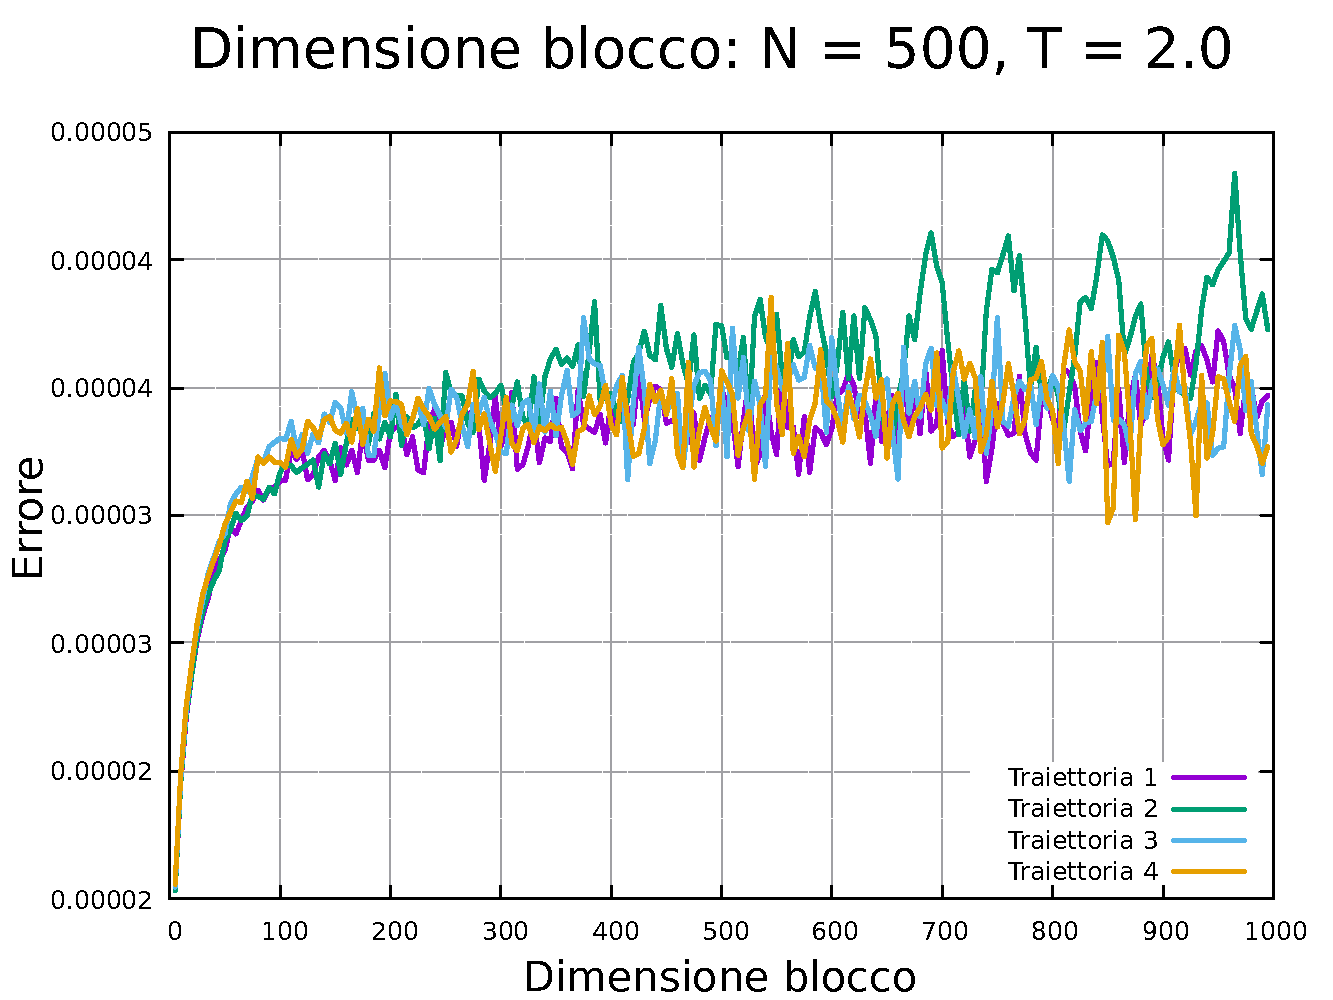
\includegraphics[width=\textwidth]{Immagini/metodiNumerici/err_500_2.0.pdf}
            \newline
            {\scriptsize Analisi per dimensione blocchi nel caso di un modello di Ising 2D.}

        \end{column}


        \begin{column}{0.45\textwidth}

            \centering
            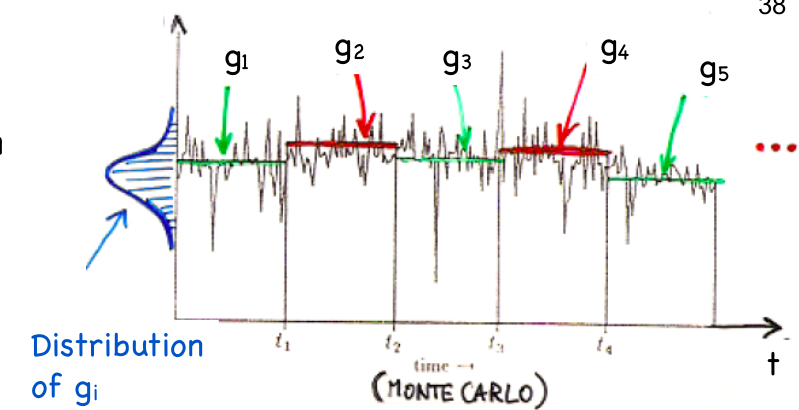
\includegraphics[width=\textwidth]{Immagini/metodiNumerici/data_blocking.png}

            \vspace{0.5cm}

            \begin{itemize}[itemsep=0.5em, label=$\diamond$]
                \item Dati raggruppati in blocchi
                \item Errore satura quando raggiunta $l_{lim}$
            \end{itemize}
            
        \end{column}
      \end{columns}
  
\end{frame}
\section{Simulazioni modello di Ising 1D}

Sono state simulate catene di spin sia in assenza che in presenza di campo magnetico. Nelle seguenti sezioni è possibile consultare 
i risultati ottenuti in entrambe le casistiche.

\newpage

\section{Conclusioni}

\begin{frame}
    \frametitle{Fine}
    \framesubtitle{}

    \begin{center}
        Grazie per l'attenzione
    \end{center}
    
\end{frame}
\section{Backup modello di Ising 1D}

%----------------------------------------%
%		       Prima slide	     	     %
%	     Osservabili per N = 1000   	 %
%----------------------------------------%
\begin{frame}
    \frametitle{Osservabili per $N_s$ = 1000, h = 0.0}
    \framesubtitle{}

    \centering
    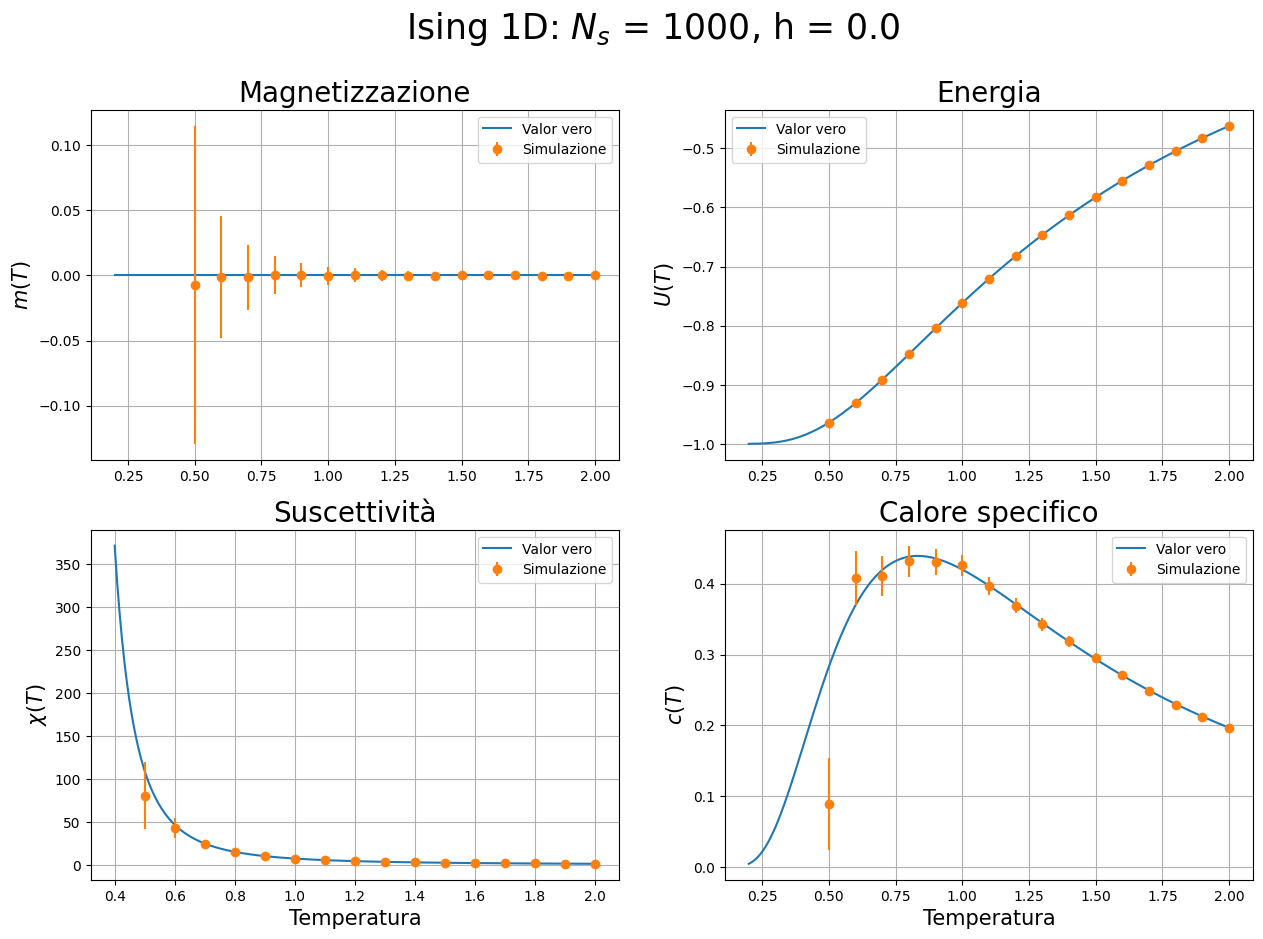
\includegraphics[width=0.65\textwidth]{Immagini/backupIsing1D/obs_1000_0.0.png}

\end{frame}



%----------------------------------------%
%		      Seconda slide	     	     %
% Differenza dal valor vero per N = 1000 %
%----------------------------------------%
\begin{frame}
    \frametitle{Differenza dal valor vero per $N_s$ = 1000, h = 0.0}
    \framesubtitle{}

    \centering
    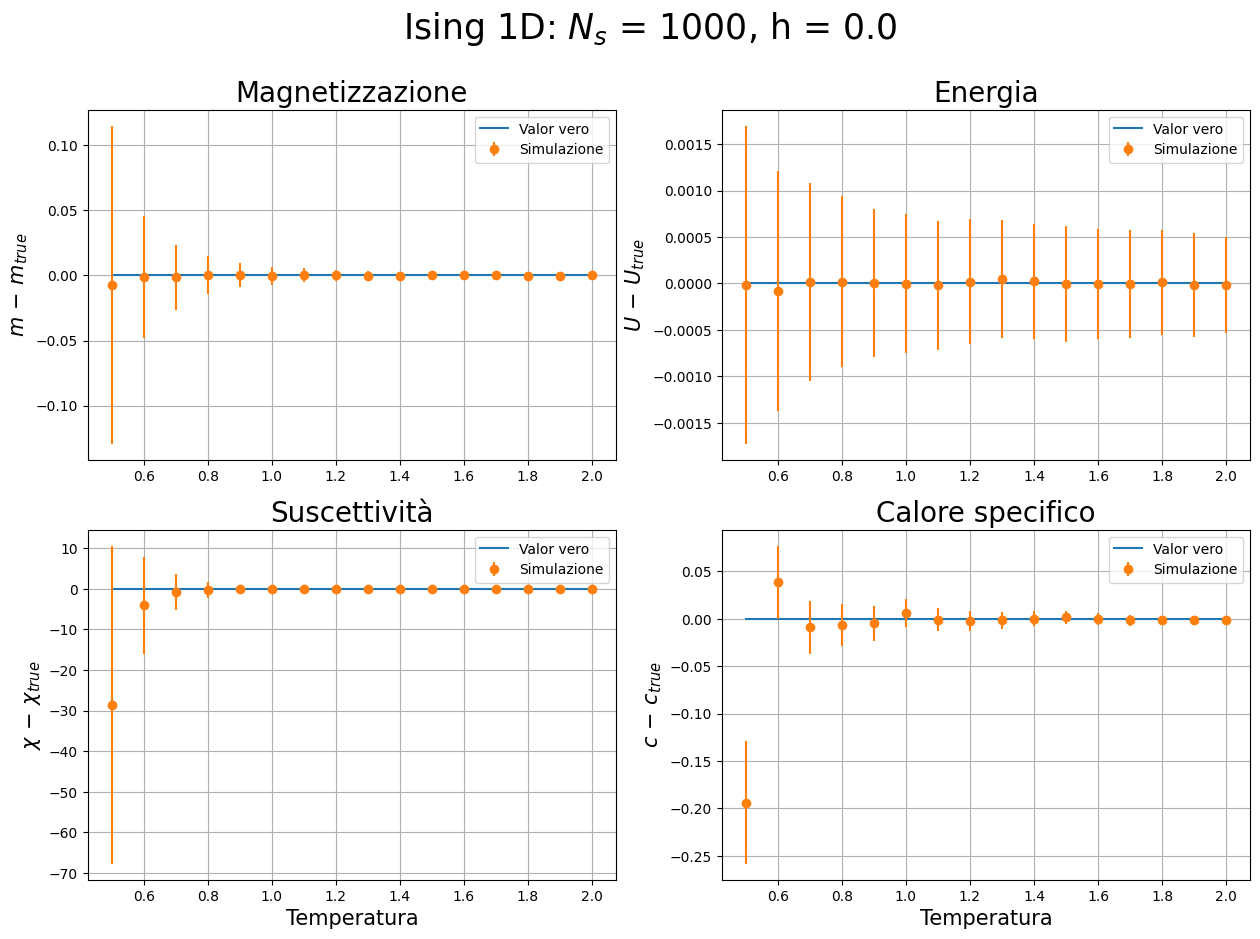
\includegraphics[width=0.65\textwidth]{Immagini/backupIsing1D/obs_1000_0.0_diff.png}

\end{frame}



%----------------------------------------%
%		       Terza slide	     	     %
%	     Osservabili per N = 3000   	 %
%----------------------------------------%
\begin{frame}
    \frametitle{Osservabili per $N_s$ = 3000, h = 0.0}
    \framesubtitle{}

    \centering
    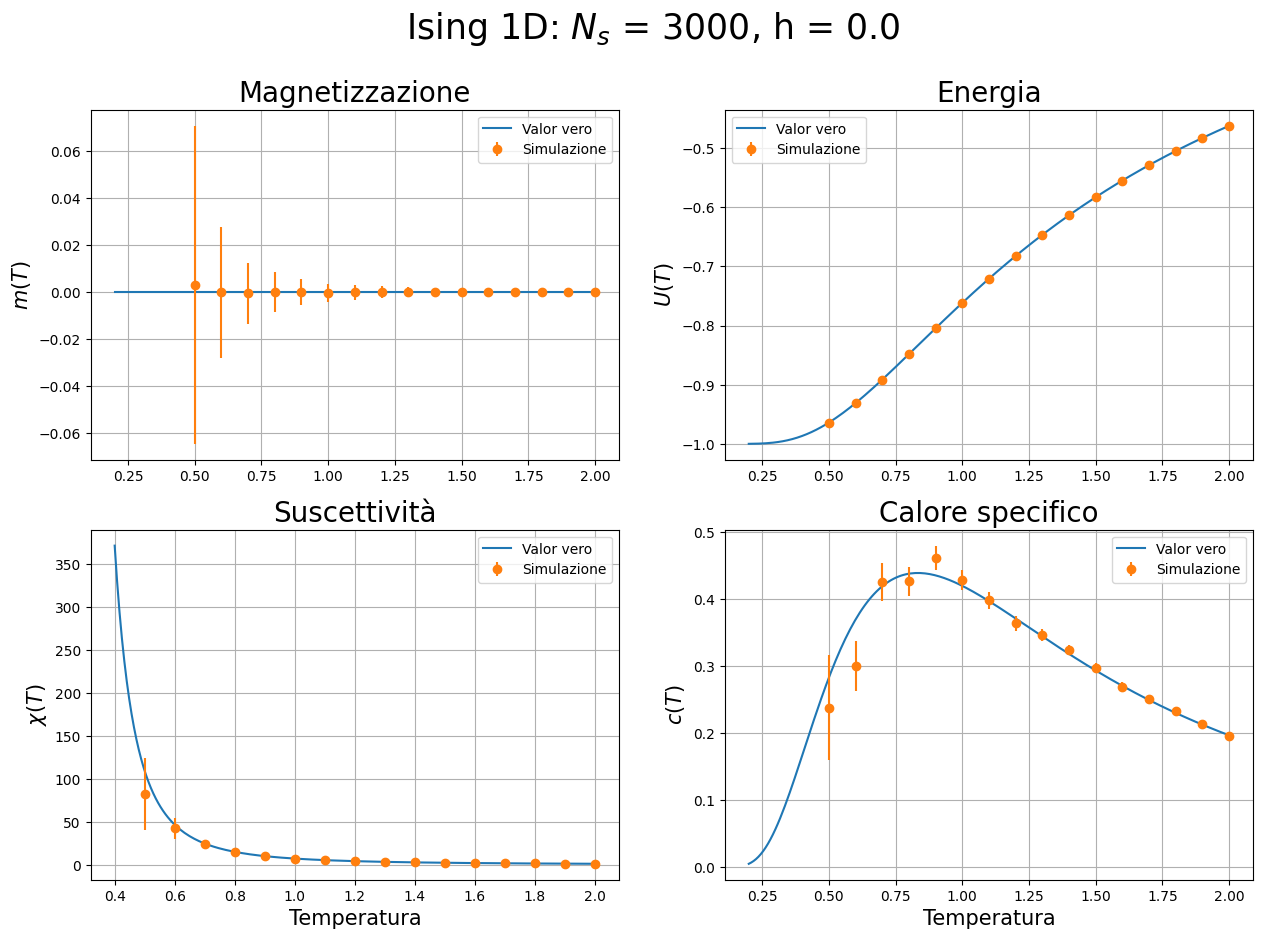
\includegraphics[width=0.65\textwidth]{Immagini/backupIsing1D/obs_3000_0.0.png}

\end{frame}



%----------------------------------------%
%		       Quarta slide	     	     %
% Differenza dal valor vero per N = 3000 %
%----------------------------------------%
\begin{frame}
    \frametitle{Differenza dal valor vero per $N_s$ = 3000, h = 0.0}
    \framesubtitle{}

    \centering
    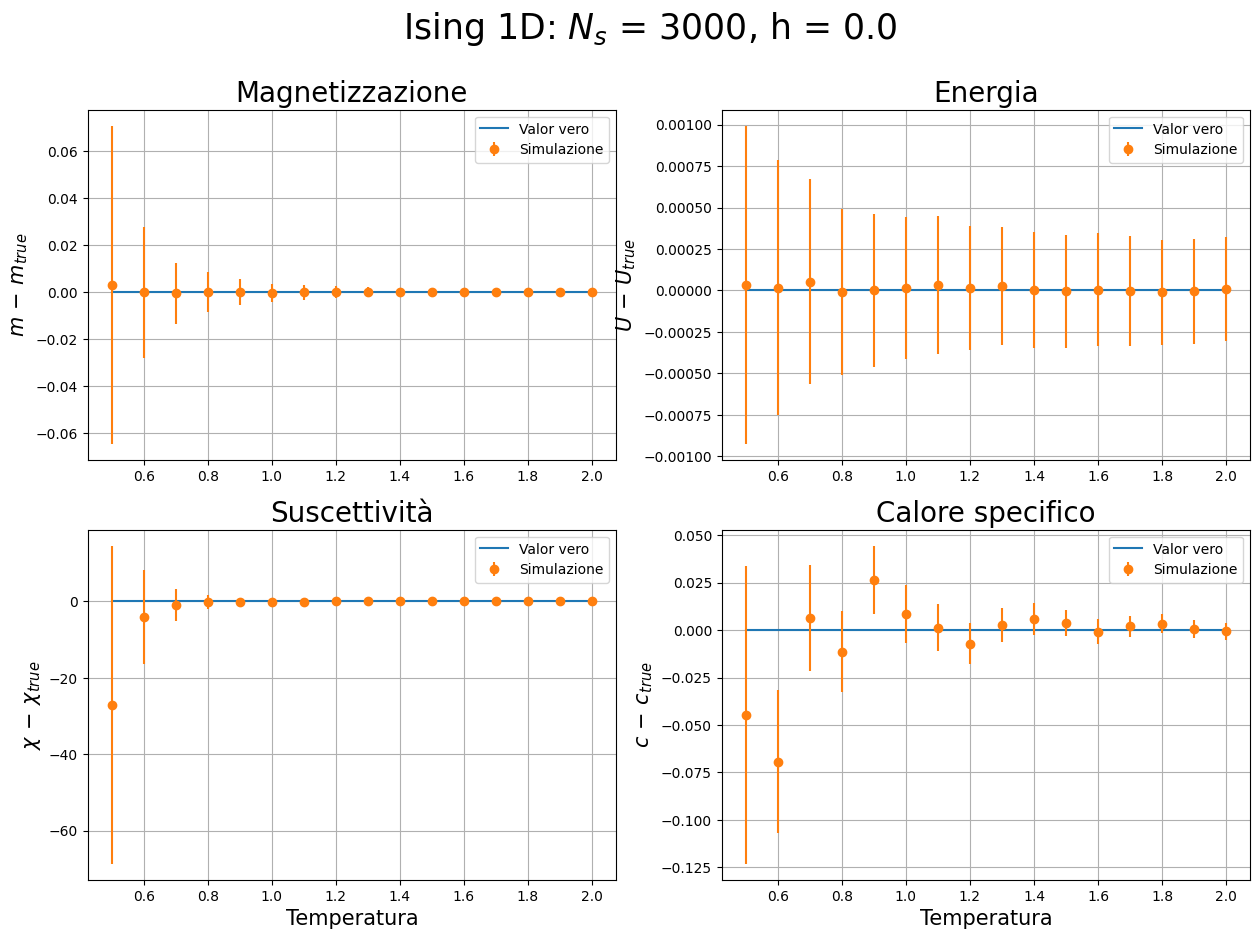
\includegraphics[width=0.65\textwidth]{Immagini/backupIsing1D/obs_3000_0.0_diff.png}

\end{frame}



%----------------------------------------%
%		       Quinta slide	     	     %
%	     Osservabili per N = 6000   	 %
%----------------------------------------%
\begin{frame}
    \frametitle{Osservabili per $N_s$ = 6000, h = 0.0}
    \framesubtitle{}

    \centering
    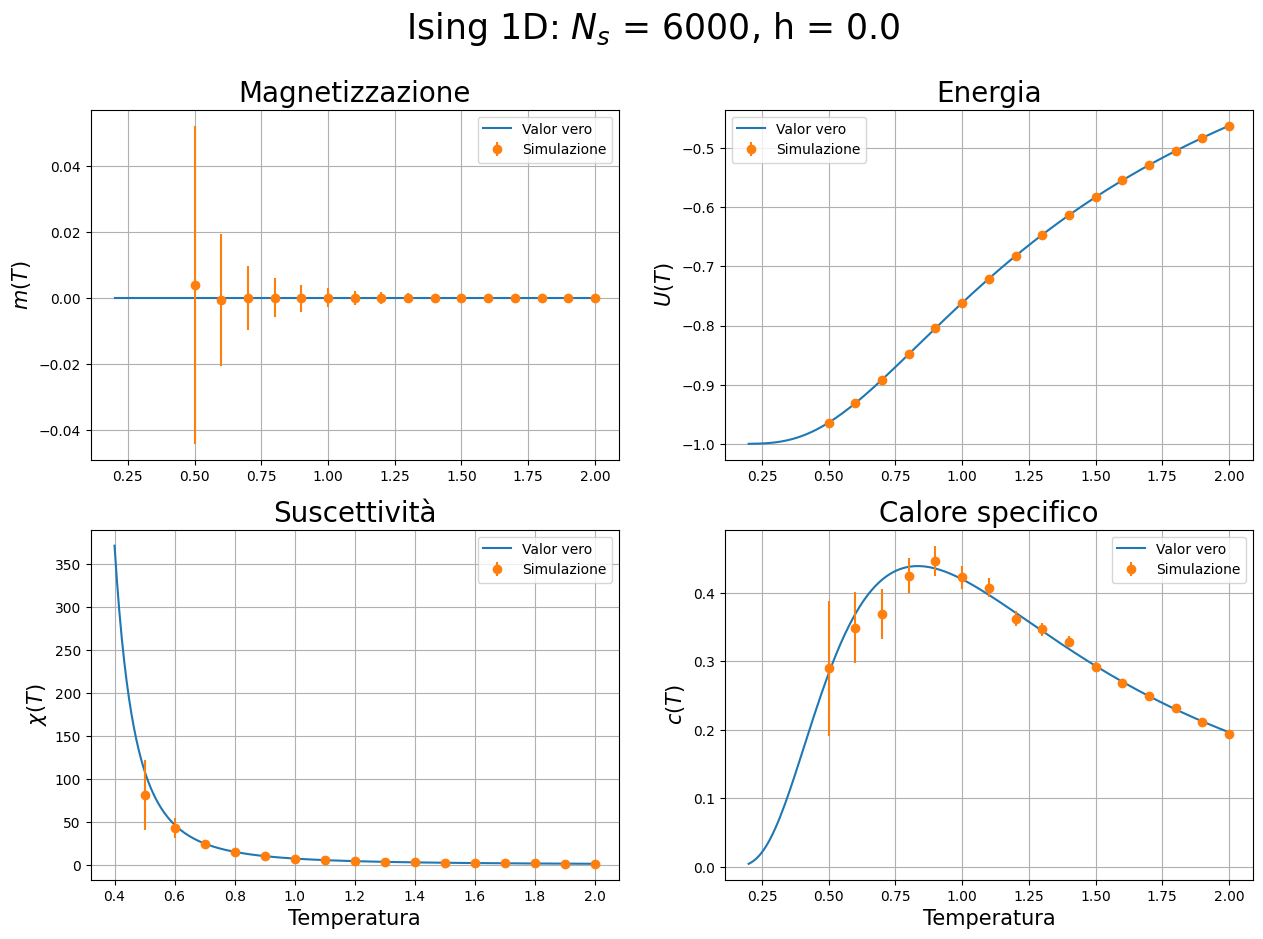
\includegraphics[width=0.65\textwidth]{Immagini/backupIsing1D/obs_6000_0.0.png}

\end{frame}



%----------------------------------------%
%		       Sesta slide	     	     %
% Differenza dal valor vero per N = 6000 %
%----------------------------------------%
\begin{frame}
    \frametitle{Differenza dal valor vero per $N_s$ = 6000, h = 0.0}
    \framesubtitle{}

    \centering
    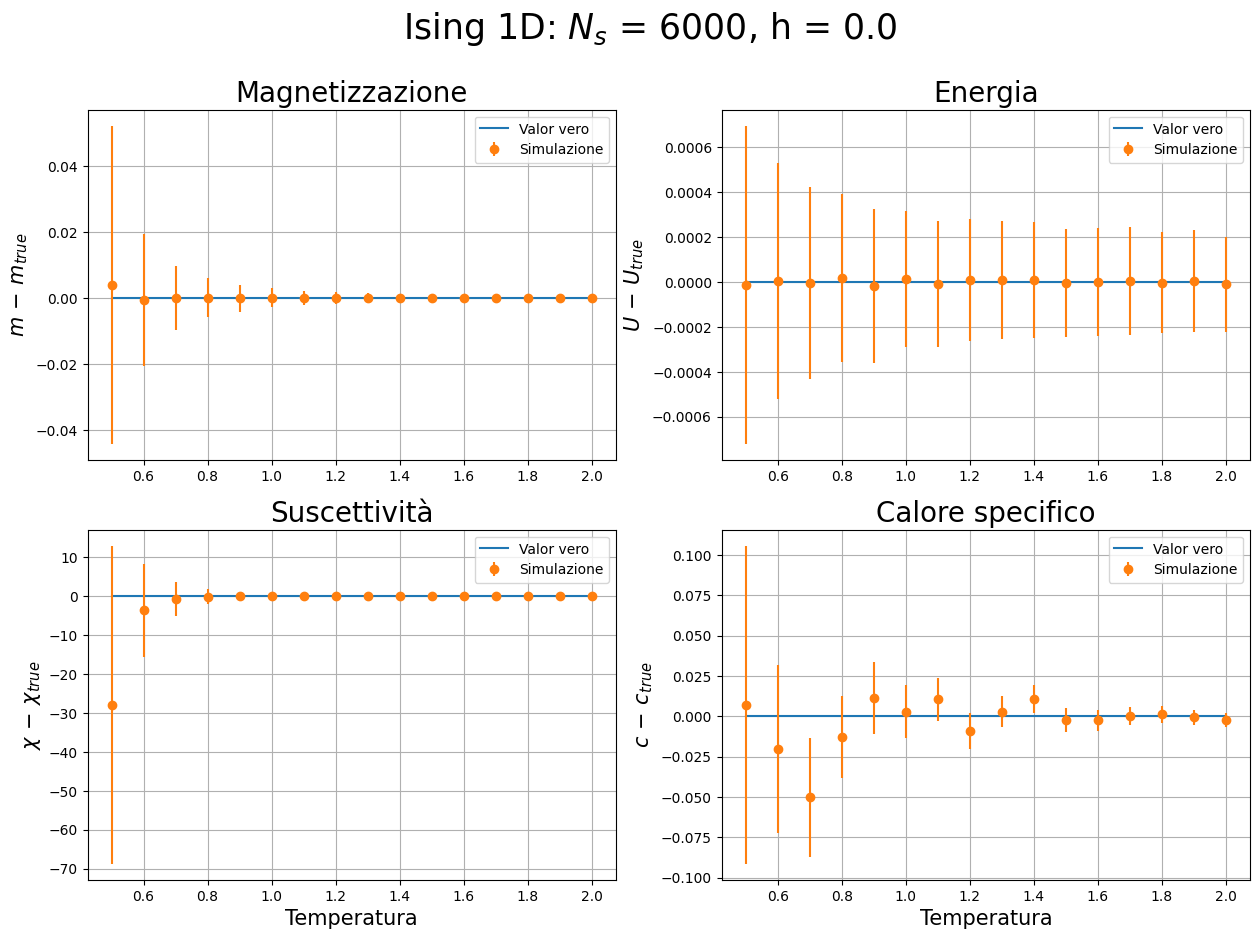
\includegraphics[width=0.65\textwidth]{Immagini/backupIsing1D/obs_6000_0.0_diff.png}

\end{frame}



%----------------------------------------%
%		      Settima slide	     	     %
%	     Osservabili per N = 10000   	 %
%----------------------------------------%
\begin{frame}
    \frametitle{Osservabili per $N_s$ = 10000, h = 0.0}
    \framesubtitle{}

    \centering
    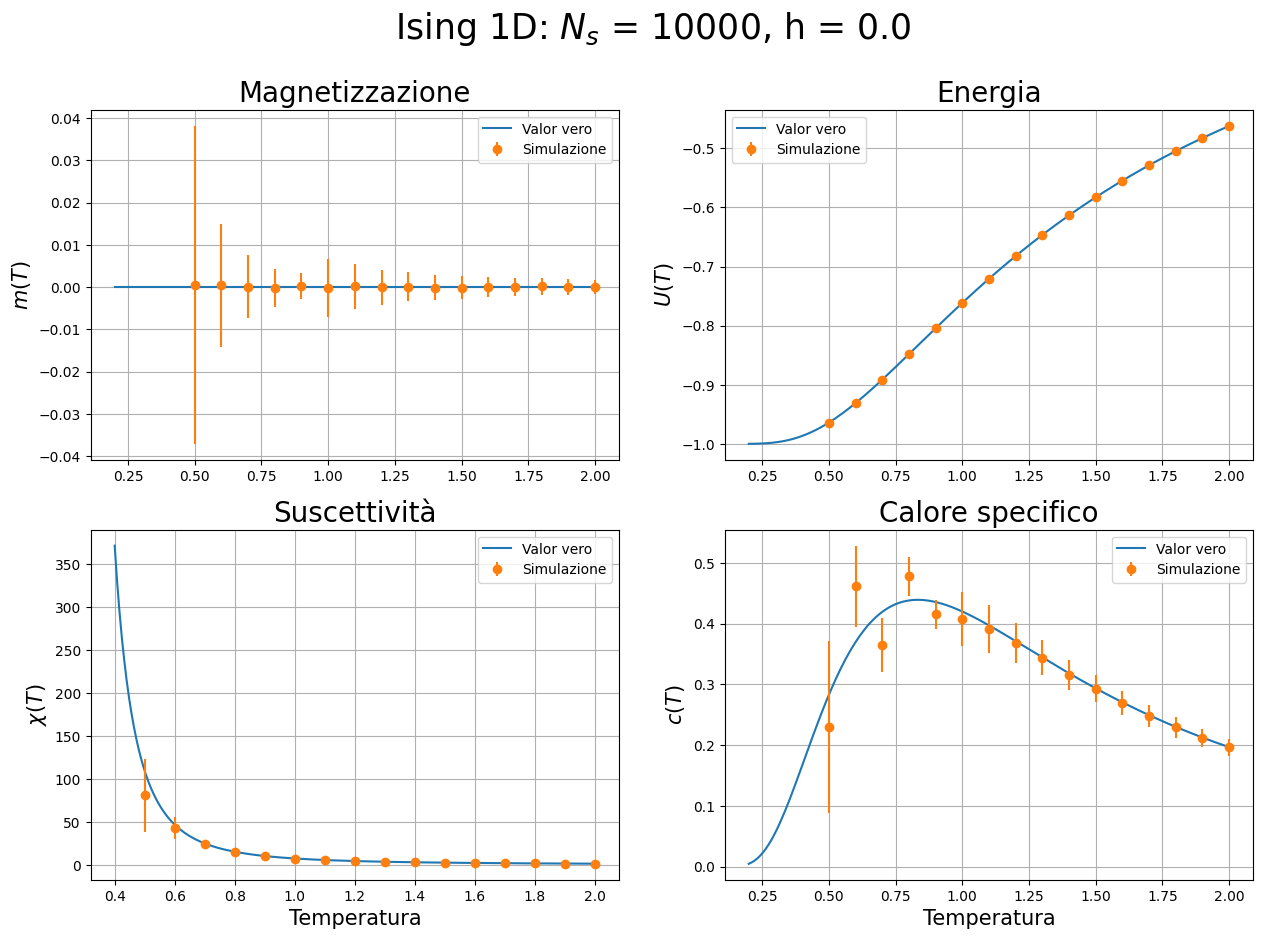
\includegraphics[width=0.65\textwidth]{Immagini/backupIsing1D/obs_10000_0.0.png}

\end{frame}



%-----------------------------------------%
%		       Ottava slide	     	      %
% Differenza dal valor vero per N = 10000 %
%-----------------------------------------%
\begin{frame}
    \frametitle{Differenza dal valor vero per $N_s$ = 10000, h = 0.0}
    \framesubtitle{}

    \centering
    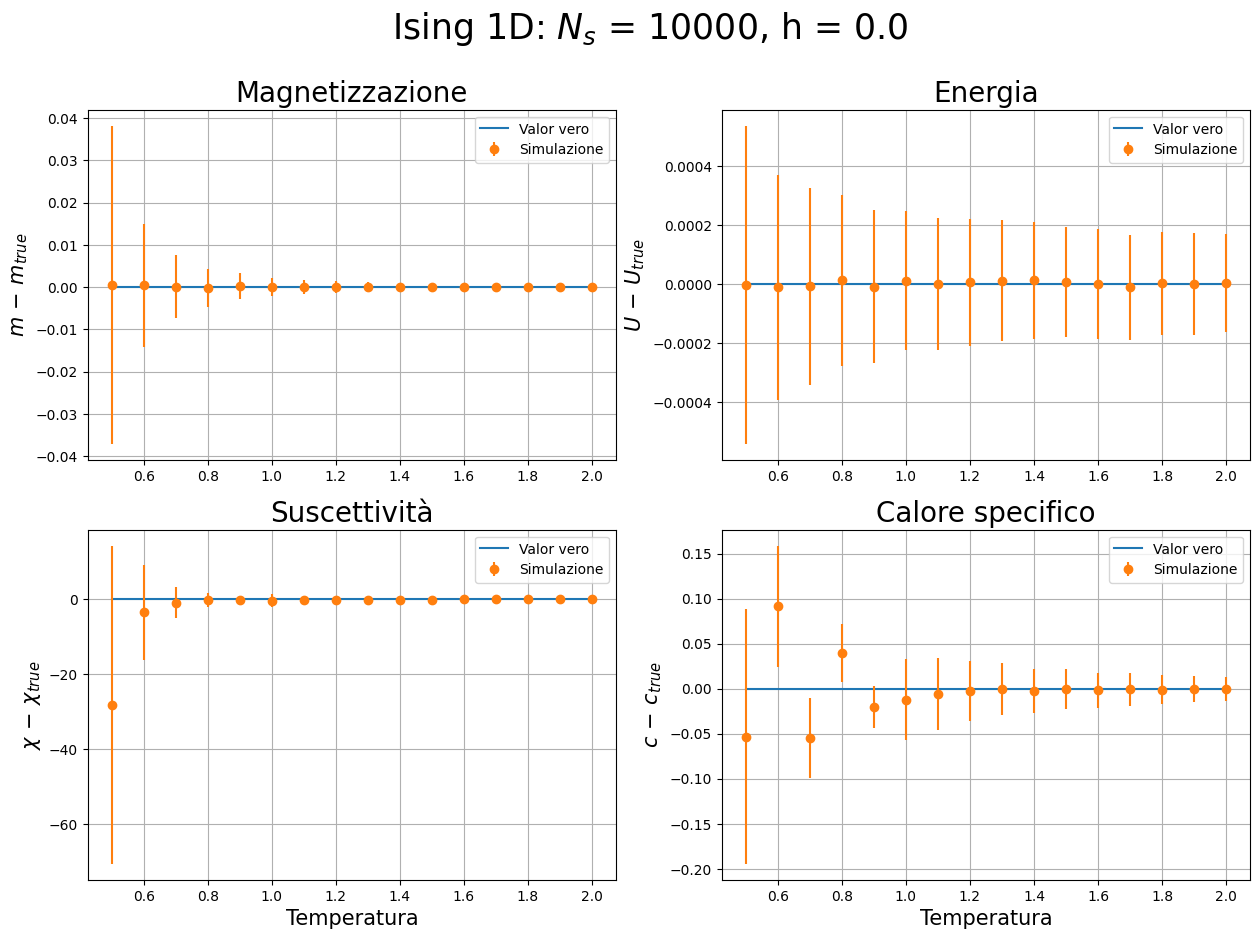
\includegraphics[width=0.65\textwidth]{Immagini/backupIsing1D/obs_10000_0.0_diff.png}

\end{frame}



%----------------------------------------%
%		       Nona slide	     	     %
%	     Osservabili per N = 1000   	 %
%----------------------------------------%
\begin{frame}
    \frametitle{Osservabili per $N_s$ = 1000, h = 0.02}
    \framesubtitle{}

    \centering
    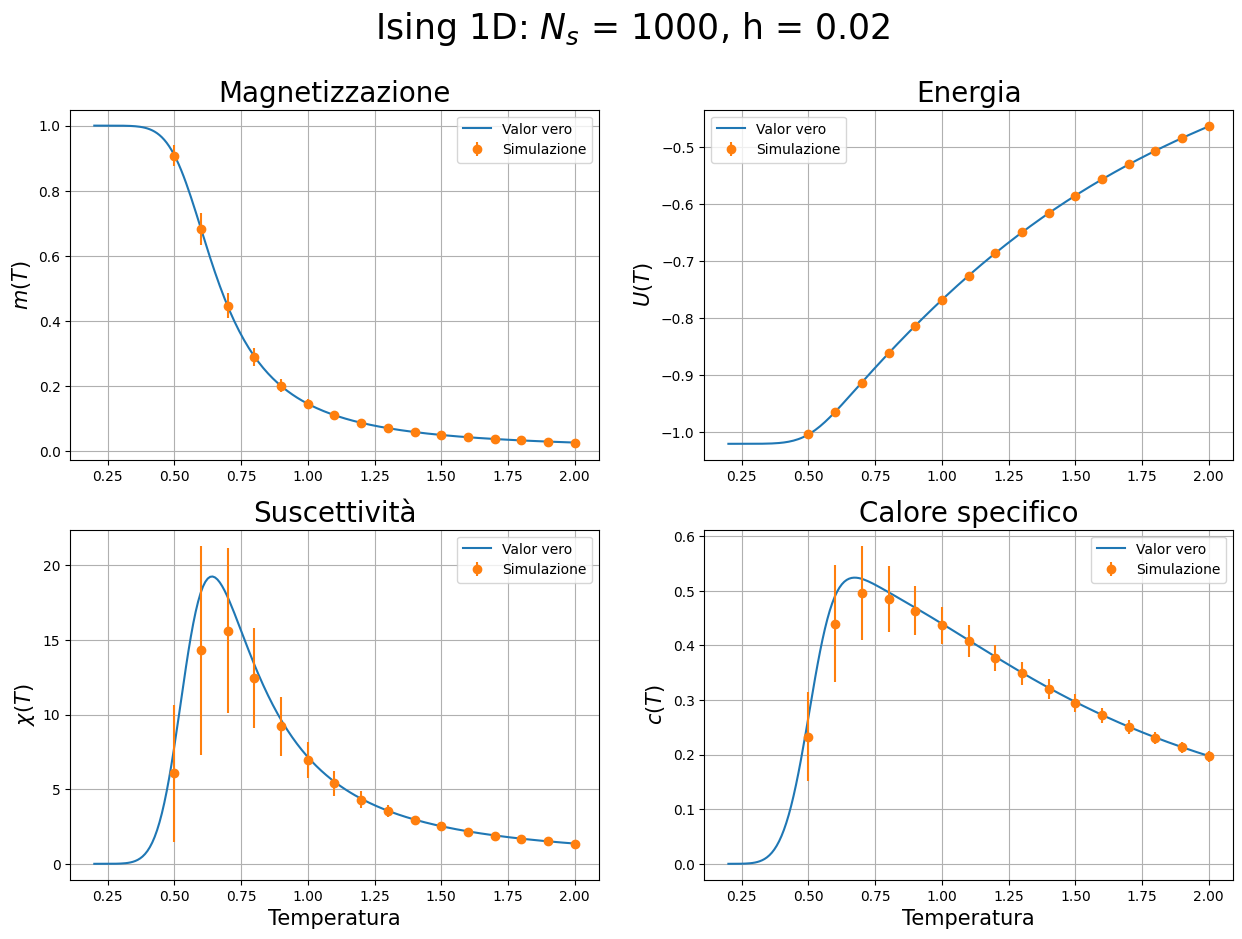
\includegraphics[width=0.65\textwidth]{Immagini/backupIsing1D/obs_1000_0.02.png}

\end{frame}



%----------------------------------------%
%		      Decima slide	     	     %
% Differenza dal valor vero per N = 1000 %
%----------------------------------------%
\begin{frame}
    \frametitle{Differenza dal valor vero per $N_s$ = 1000, h = 0.02}
    \framesubtitle{}

    \centering
    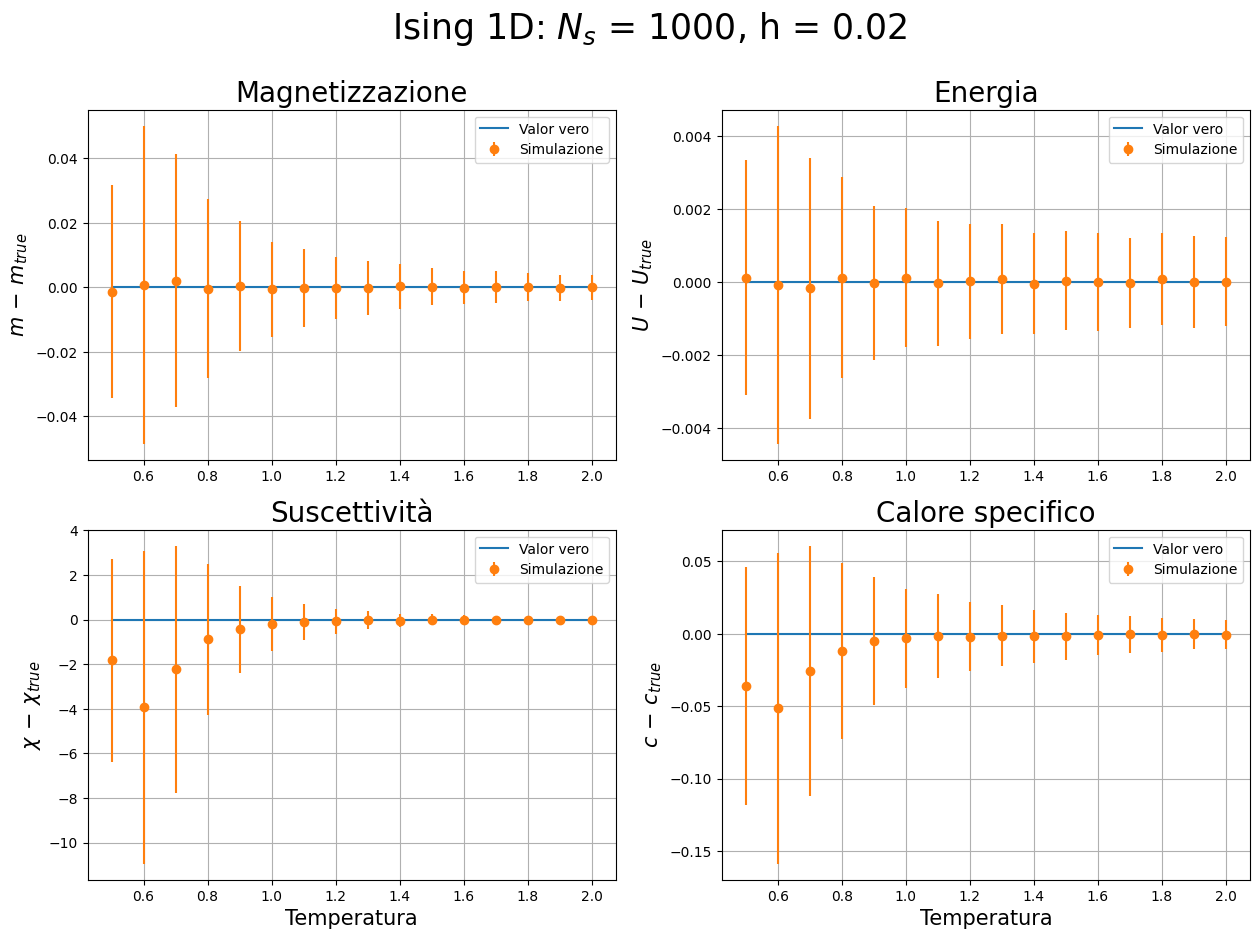
\includegraphics[width=0.65\textwidth]{Immagini/backupIsing1D/obs_1000_0.02_diff.png}

\end{frame}



%----------------------------------------%
%		     Undicesima slide	     	 %
%	     Osservabili per N = 3000   	 %
%----------------------------------------%
\begin{frame}
    \frametitle{Osservabili per $N_s$ = 3000, h = 0.02}
    \framesubtitle{}

    \centering
    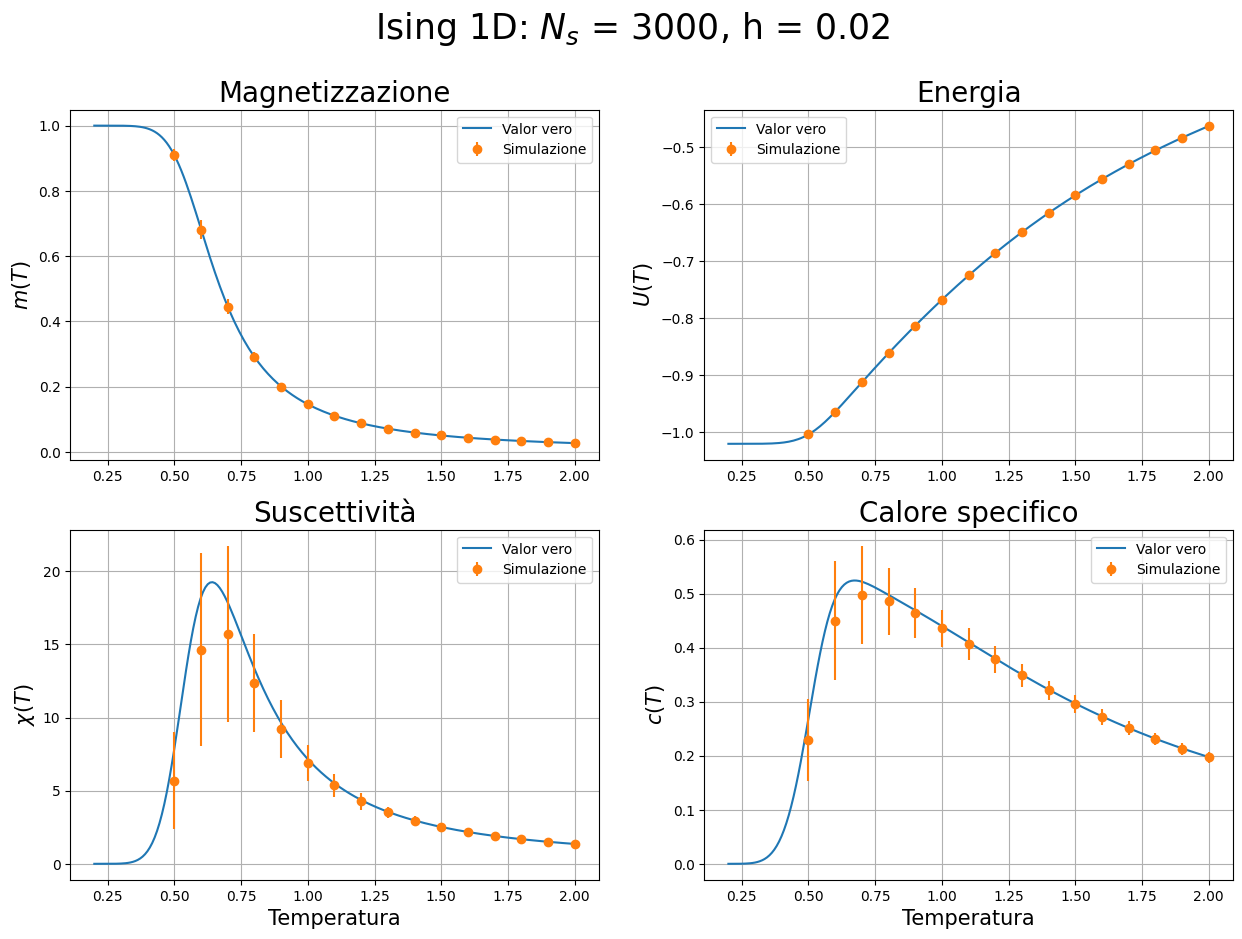
\includegraphics[width=0.65\textwidth]{Immagini/backupIsing1D/obs_3000_0.02.png}

\end{frame}



%----------------------------------------%
%		    Dodicesima slide    	     %
% Differenza dal valor vero per N = 3000 %
%----------------------------------------%
\begin{frame}
    \frametitle{Differenza dal valor vero per $N_s$ = 3000, h = 0.02}
    \framesubtitle{}

    \centering
    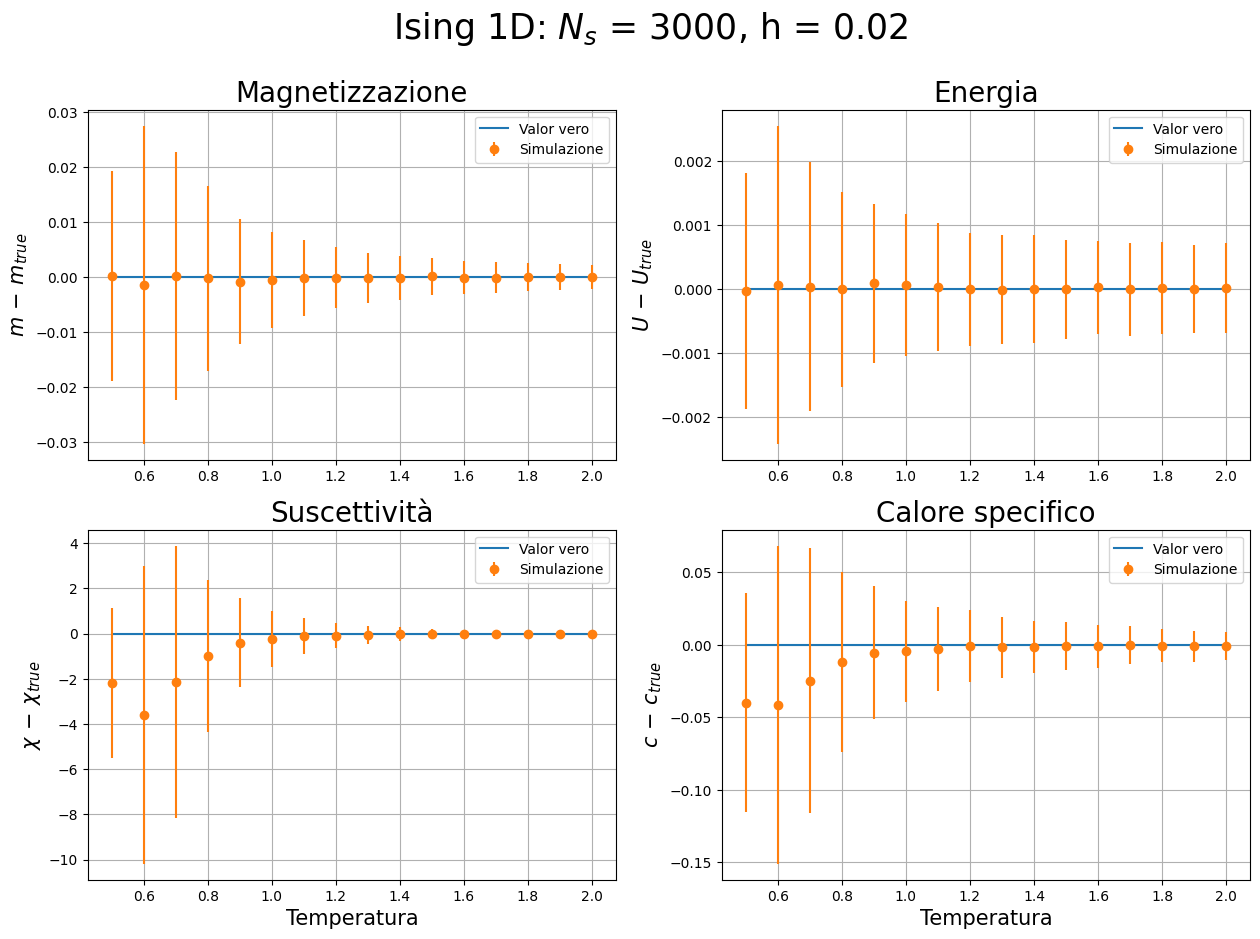
\includegraphics[width=0.65\textwidth]{Immagini/backupIsing1D/obs_3000_0.02_diff.png}

\end{frame}



%----------------------------------------%
%		     Tredicesima slide	         %
%	     Osservabili per N = 6000   	 %
%----------------------------------------%
\begin{frame}
    \frametitle{Osservabili per $N_s$ = 6000, h = 0.02}
    \framesubtitle{}

    \centering
    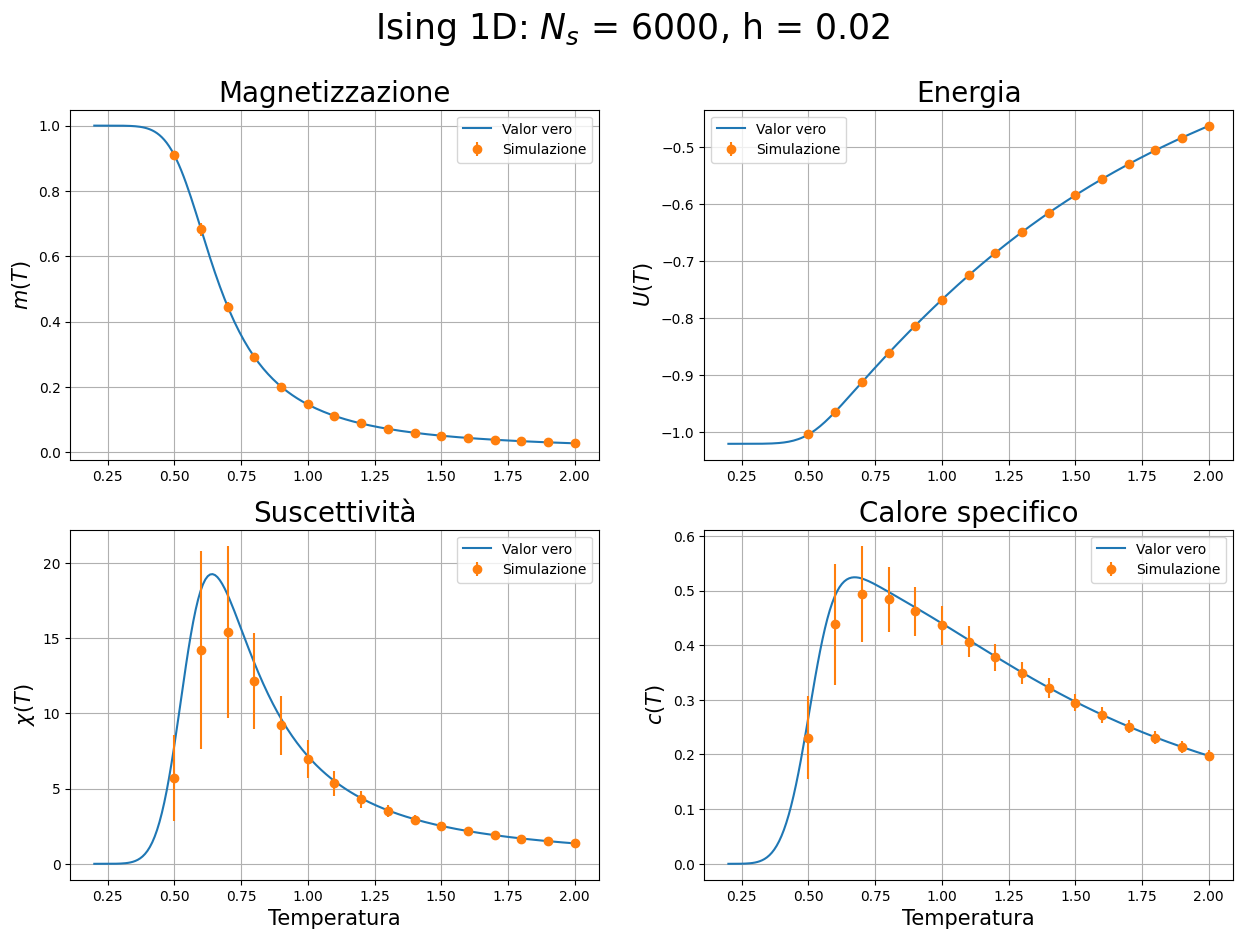
\includegraphics[width=0.65\textwidth]{Immagini/backupIsing1D/obs_6000_0.02.png}

\end{frame}



%----------------------------------------%
%		  Quattordicesima slide	     	 %
% Differenza dal valor vero per N = 6000 %
%----------------------------------------%
\begin{frame}
    \frametitle{Differenza dal valor vero per $N_s$ = 6000, h = 0.02}
    \framesubtitle{}

    \centering
    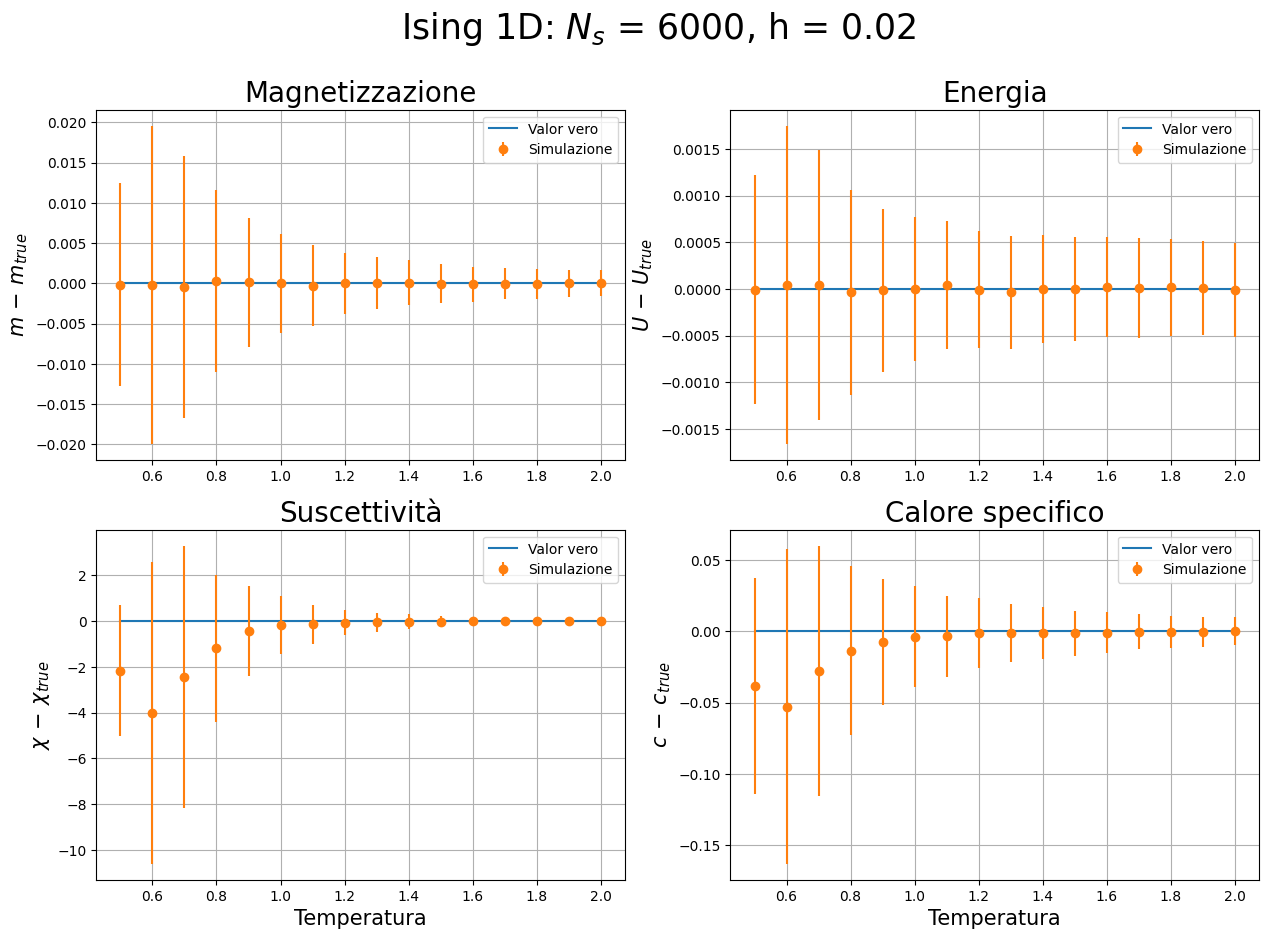
\includegraphics[width=0.65\textwidth]{Immagini/backupIsing1D/obs_6000_0.02_diff.png}

\end{frame}



%----------------------------------------%
%		     Quindicesima slide	     	 %
%	     Osservabili per N = 10000   	 %
%----------------------------------------%
\begin{frame}
    \frametitle{Osservabili per $N_s$ = 10000, h = 0.02}
    \framesubtitle{}

    \centering
    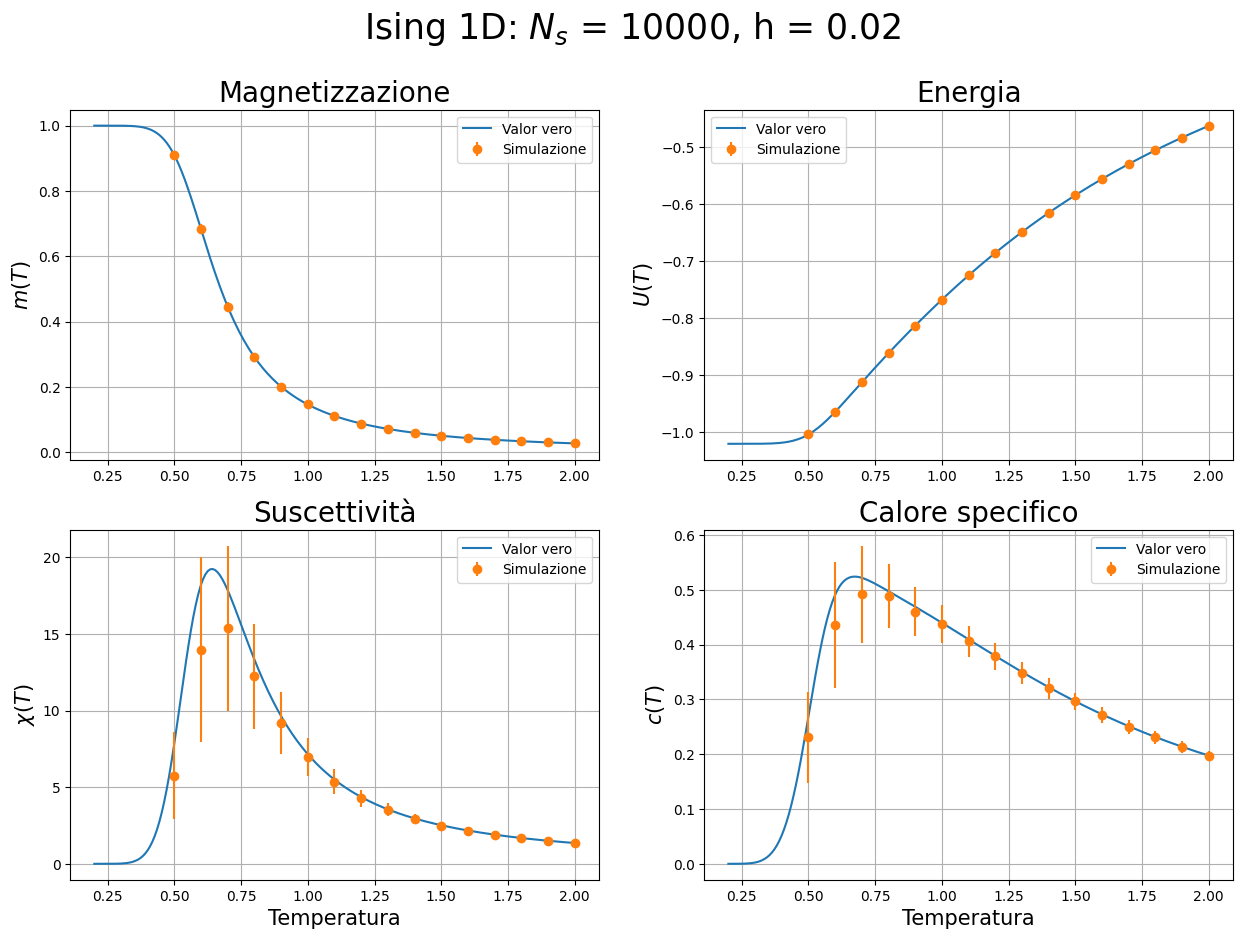
\includegraphics[width=0.65\textwidth]{Immagini/backupIsing1D/obs_10000_0.02.png}

\end{frame}



%----------------------------------------%
%		     Sedicesima slide	     	 %
%  Differenza dal valor vero, N = 10000  %
%----------------------------------------%
\begin{frame}
    \frametitle{Differenza dal valor vero per $N_s$ = 10000, h = 0.02}
    \framesubtitle{}

    \centering
    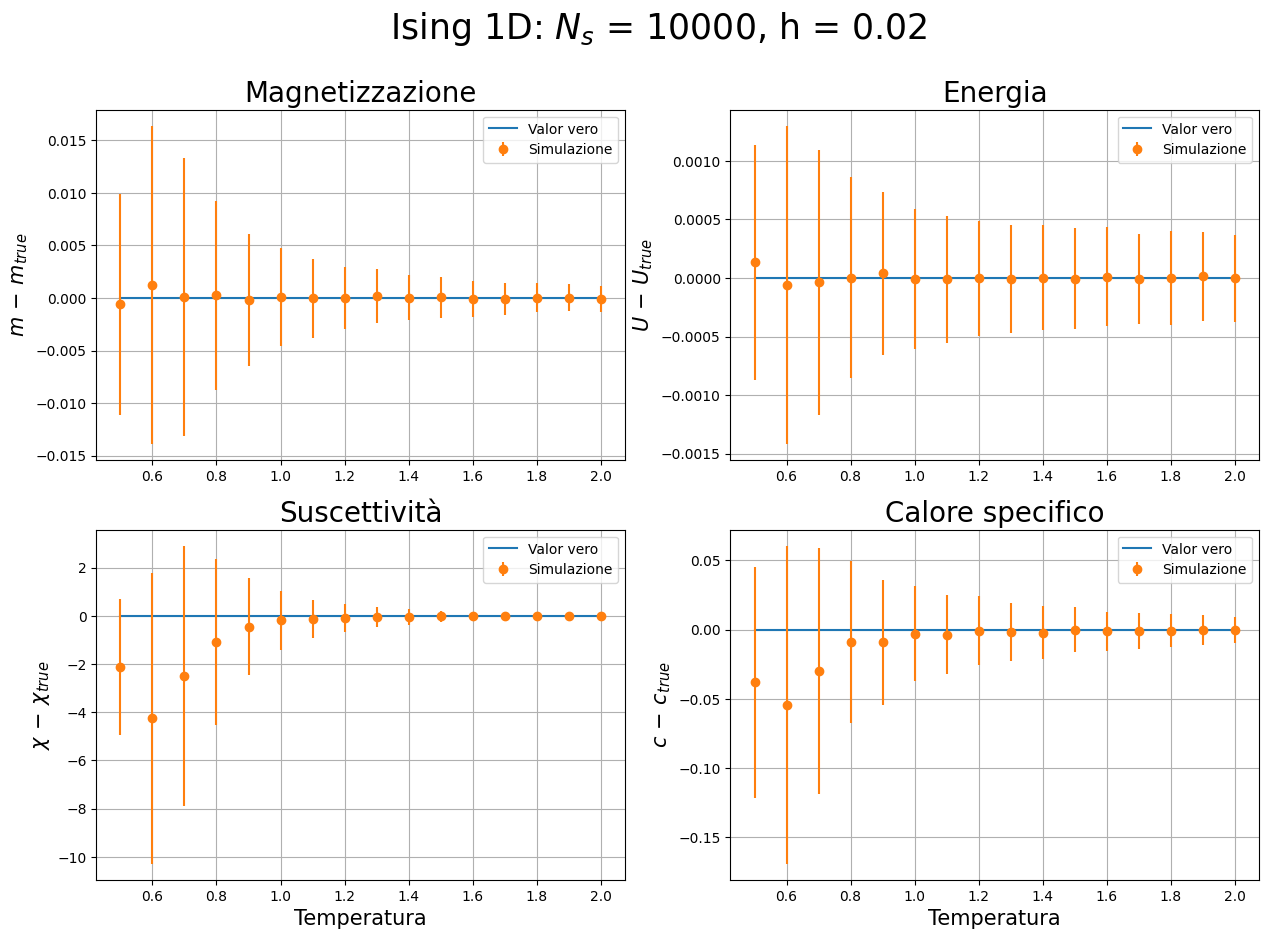
\includegraphics[width=0.65\textwidth]{Immagini/backupIsing1D/obs_10000_0.02_diff.png}

\end{frame}

%----------------------------------------%
%		       Prima slide	     	     %
%	Osservabili per reticolo 100 x 100   %
%----------------------------------------%
\begin{frame}
    \frametitle{Osservabili per reticolo $100 \times 100$}
    \framesubtitle{Ising 2D}

    \centering
    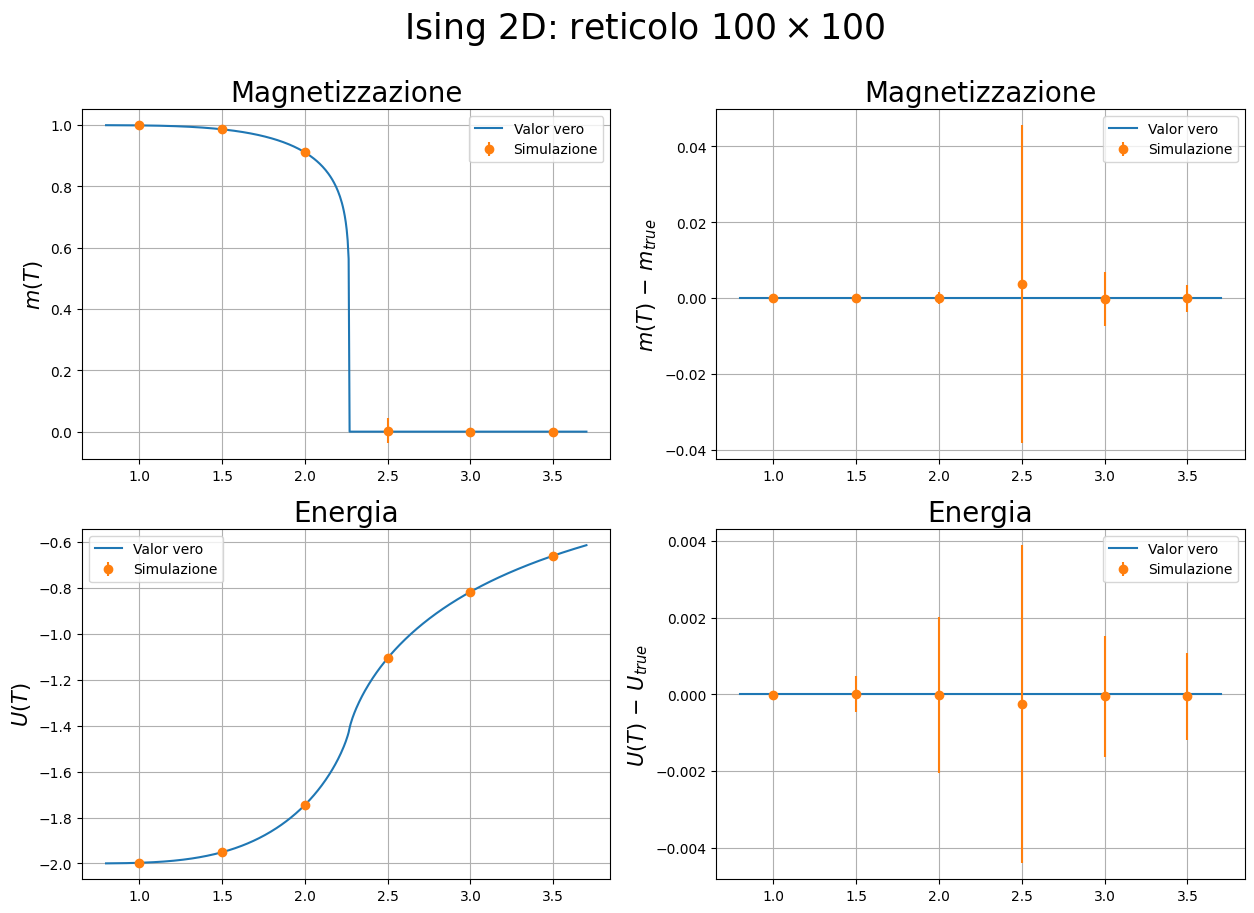
\includegraphics[width=0.65\textwidth]{Immagini/backupIsing2D/obs_100.png}

\end{frame}



%----------------------------------------%
%		      Seconda slide	     	     %
%	Osservabili per reticolo 100 x 100   %
%----------------------------------------%
\begin{frame}
    \frametitle{Osservabili per reticolo $200 \times 200$}
    \framesubtitle{Ising 2D}

    \centering
    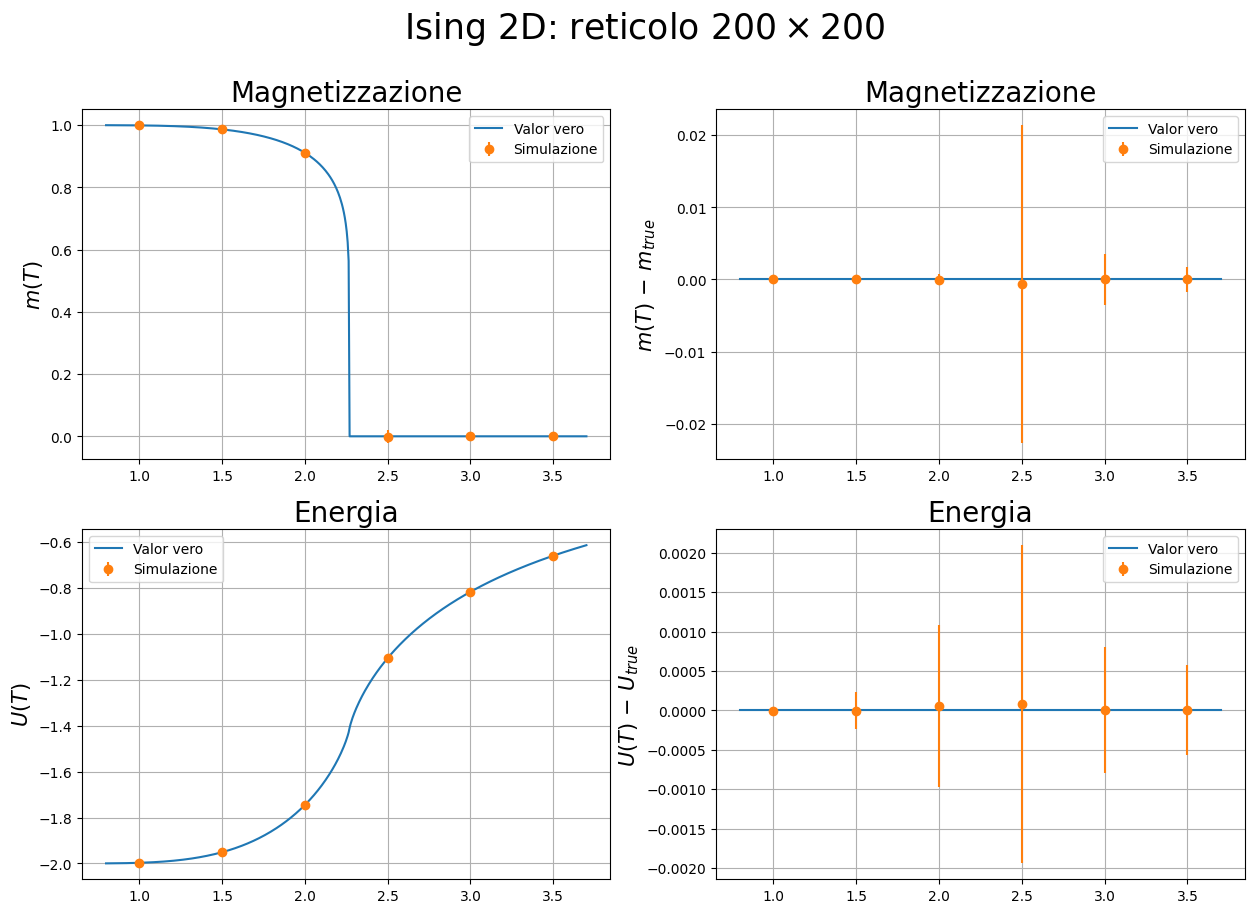
\includegraphics[width=0.65\textwidth]{Immagini/backupIsing2D/obs_200.png}

\end{frame}



%----------------------------------------%
%		       Terza slide	     	     %
%	Osservabili per reticolo 300 x 300   %
%----------------------------------------%
\begin{frame}
    \frametitle{Osservabili per reticolo $300 \times 300$}
    \framesubtitle{Ising 2D}

    \centering
    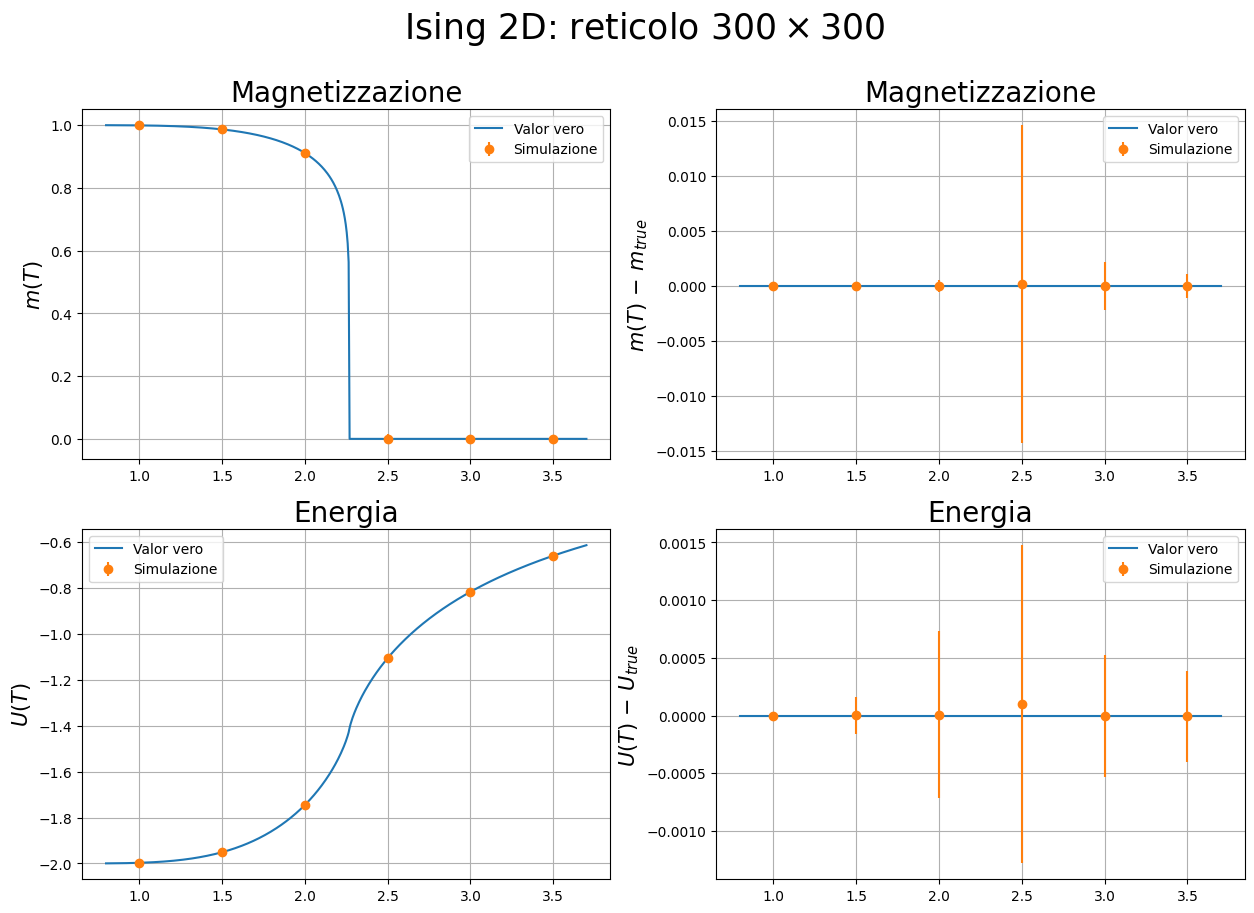
\includegraphics[width=0.65\textwidth]{Immagini/backupIsing2D/obs_300.png}

\end{frame}



%----------------------------------------%
%		       Quarta slide	     	     %
%	Osservabili per reticolo 400 x 400   %
%----------------------------------------%
\begin{frame}
    \frametitle{Osservabili per reticolo $400 \times 400$}
    \framesubtitle{Ising 2D}

    \centering
    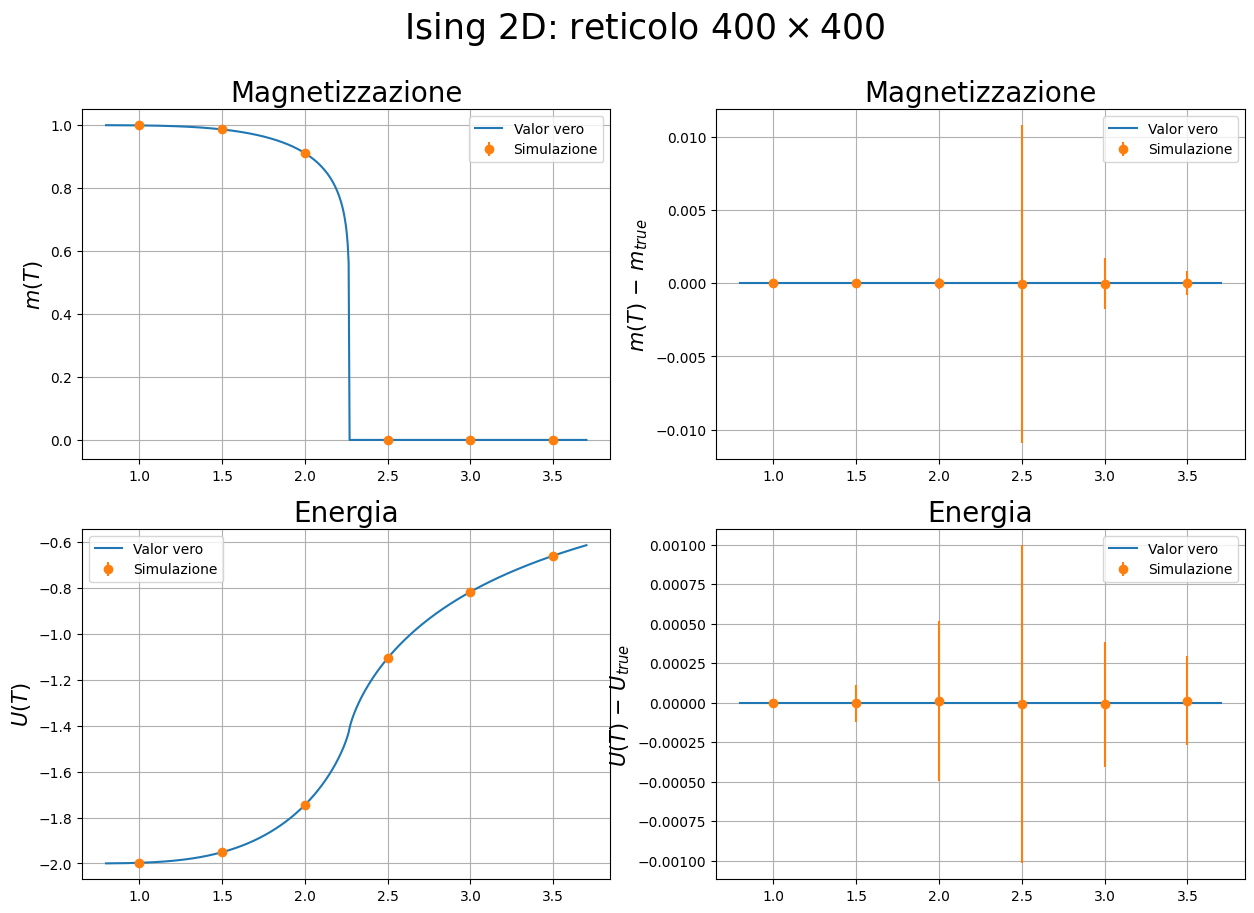
\includegraphics[width=0.65\textwidth]{Immagini/backupIsing2D/obs_400.png}

\end{frame}



%----------------------------------------%
%		       Quinta slide	     	     %
%	Osservabili per reticolo 500 x 500   %
%----------------------------------------%
\begin{frame}
    \frametitle{Osservabili per reticolo $500 \times 500$}
    \framesubtitle{Ising 2D}

    \centering
    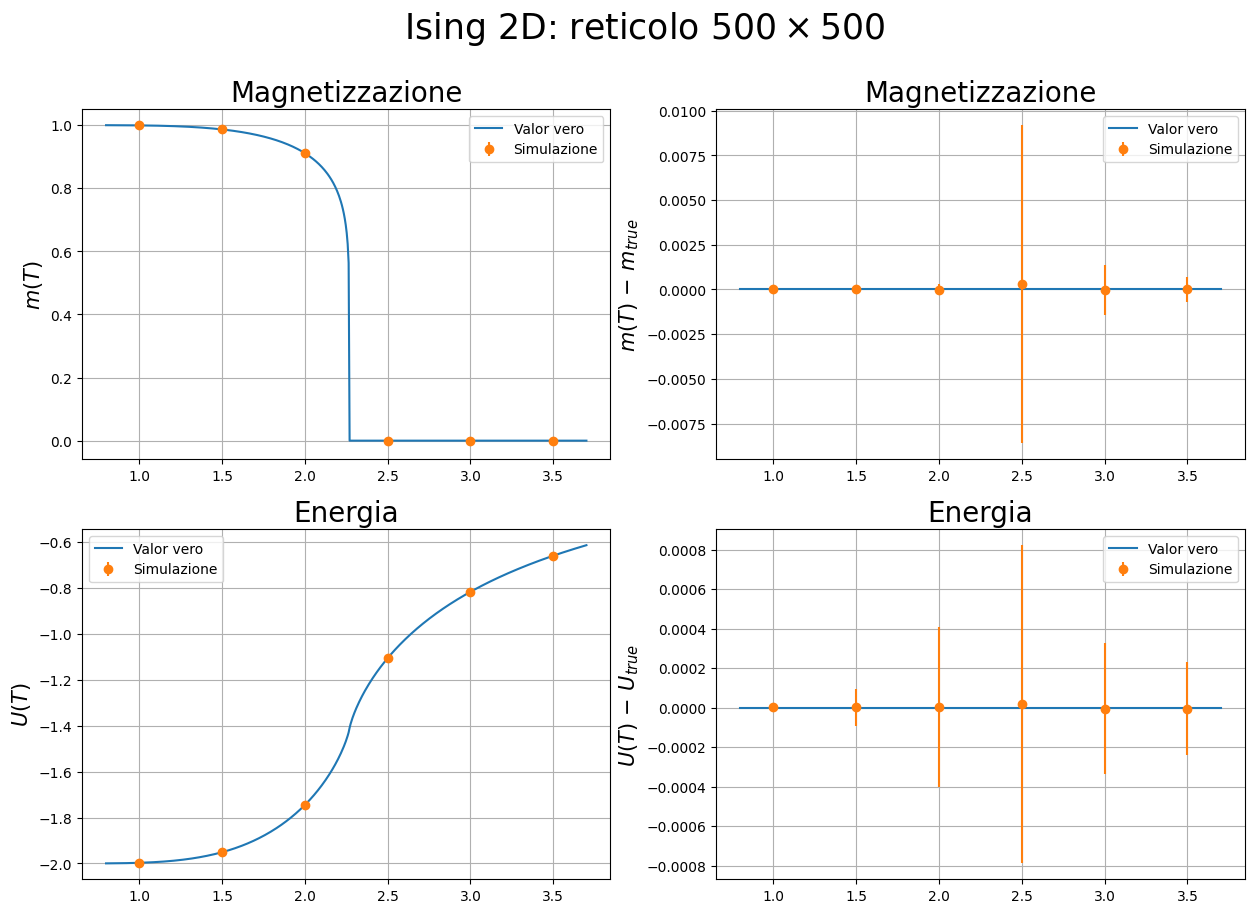
\includegraphics[width=0.65\textwidth]{Immagini/backupIsing2D/obs_500.png}

\end{frame}


\end{document}